\documentclass[10pt,oneside,onecolumn,openany]{book}
\usepackage[spanish]{babel}
\usepackage[utf8]{inputenc}
\usepackage{listings}
\usepackage{enumitem}
\usepackage{cdtBook}
\usepackage{usecases}
\usepackage{txfonts}
\usepackage{pdfpages}
\usepackage{hyperref}
\usepackage{nameref}
\usepackage{caption}
\usepackage{placeins}
\usepackage[T1]{fontenc}
\usepackage{multirow}
\usepackage{lscape}

\renewcommand\paragraph{\@startsection{paragraph}{4}{\z@}%
            {-2.5ex\@plus -1ex \@minus -.25ex}%
            {1.25ex \@plus .25ex}%
            {\normalfont\normalsize\bfseries}}
\makeatother
\setcounter{secnumdepth}{4} % how many sectioning levels to assign numbers to
\setcounter{tocdepth}{4}    % how many sectioning levels to show in ToC

%%%%%%%%%%%%%%%%%%%%%%%%%%%%%%%%%%%%%%%%%%%%%%%%%%%%%%%%%%%%%%%%
\begin{document}
%\includepdf{Portada} Inlcuir portada
\frontmatter
\tableofcontents
\listoffigures
\listoftables
\mainmatter
\LRCornerWallPaper{1}{images/Etiquetas/bssnvo}

%=========================================================
\chapter{Introducción}
\label{cap:Introducción}
Este documento contiene las especificaciones del proyecto Directorio que corresponde al trabajo realizado durante 2019, para (INDICAR) redactado por parte del equipo de TI de la \textbf{División de Innovación Educativa}.
%---------------------------------------------------------

\section{Presentación}
El crecimiento de las empresas y negocios tiene como consecuencia primordial el aumento de información, mientras la organización crezca la información también aumenta, sería más difícil mantenerla, manejarla y controlarla. Por lo que surge la necesidad de manejar estos grandes volúmenes de datos de un forma más fácil y automatizada con aplicaciones informáticas que nos faciliten dichas labores.
\\\\
El presente documento detalla la solución propuesta para la Gestión de la información que maneja el ``IMSS" que en este caso será de las \hyperlink{Glo:Delegaciones}{Delegaciones} y \hyperlink{Glo:UMAE}{UMAES}.
\\\\
Se propone una gestión mejorada mediante un sistema web que automatice las operaciones que se requieran para la gestión de espectaculares.
\\\\
Este documento tiene distintos propósitos, los cuales incluyen:
\begin{itemize}
    \item Mostrar los distintos tipos de requerimientos del sistema que se van a desarrollar a lo largo del semestre.
    \item Mostrar los avances y características que se vayan agregando al sistema para una mejor comprensión de la información de los directorios, describiendo los puntos de vista y acciones que se llevaran a cabo en la construcción de dicho sistema.
    \item El presente documento se usará como medio de aprobación o rechazo del sistema que se está realizando.
\end{itemize}

\section{Organización del contenido}
En el capítulo \ref{cap:Introducción} es la parte dónde se define el contexto actual del manejo del directorio de los empleados en el IMSS. En este apartado se incluye una introducción, la organización del contenido, así como la organización de los requerimientos de usuario, requerimientos funcionales, reglas de negocio, procedimientos, casos de uso e interfaces de usuario. \\

En el capítulo \ref{cap:Glosario} es la parte dónde se define el conjunto de términos que estaremos utilizando a lo largo de todo el documento, el organigrama del IMSS, además de la definición de los usuarios que utilizarán el sistema, así como sus responsabilidades, perfil del empleado y procesos en los que participa. \\

En el capítulo \ref{cap:Propuesta} es la parte del análisis del problema y el contexto al que nos estamos enfrentando. En este apartado se definen los requisitos de usuario, lo cuales nos permiten conocer cuales son las necesidades de éste, de igual manera se define la propuesta de solución, los objetivos generales y específicos, descripción de la solución a realizar. \\

En el capítulo \ref{cap:ModeloDinamico} es la parte que nos dará un mejor contexto de como se formará el sistema después de haber hecho el análisis, aquí pretendemos dar a conocer por medio del uso de los casos de uso cual será el comportamiento del sistema.

En el capítulo \ref{cap:ModeloDeLaInteraccion} se dará la descripción de las pantallas que conformaran el sistema. Cada pantalla contiene un objetivo, el diseño que contiene, las salidas que vamos a observar en dicha pantalla, así como las entradas que contendrá cada una de ellas. \\

En el capítulo \ref{cap:ModeloEstatico} se dará la descripción de en que lenguaje de programación, se programara el sistema, las características del servidor en cuando a hardware y software para poder correr el sistema y también como estará compuestos los objetos en el diagrama de clases sus atributos, métodos, relaciones, etc. \\

En el capítulo \ref{cap:DiseniodeInformacion} se dará la descripción de como estará conformada la estructura de la base de datos, como estarán conformados los metadatos en la base de datos y como están conformadas las consultas en el sistema para hacer la selección especifica de los datos que se necesitan en su momento\\

En el capítulo \ref{cap:CasosDePrueba} se dará la descripción de como las estarán estructuradas las pruebas que se harán en el sistema así como en comportamiento que se tiene contemplado que hará el sistema al momento de realizar una prueba especifica. \\

\section{Notación, símbolos y convenciones utilizadas}
\setlength{\parindent}{0cm}
Los requerimientos del usuario utilizan una clave XX-RUX, donde:
    
\begin{description}
    \item[RU] Es la clave para todos los {\bf R}equerimientos del {\bf U}suario.
    \item[X] Es un número consecutivo: 1, 2, 3, ...
    \item[xx]  Son las abreviaciones de los actores que usaran el sistema.
\end{description}

 Los requerimientos funcionales utilizan una clave RFX, donde:
    
\begin{description}
    \item[RF] Es la clave para todos los {\bf R}equerimientos {\bf F}uncionales
    \item[X] Es un número consecutivo: 1, 2, 3, ...
\end{description}

 Los requerimientos no funcionales utilizan una clave RNFX, donde:
    
\begin{description}
    \item[RNF] Es la clave para todos los {\bf R}equerimientos {\bf N}o {\bf F}uncionales
    \item[X] Es un número consecutivo: 1, 2, 3, ...
\end{description}

Las reglas del negocio utilizan una clave BRX, donde:
    
\begin{description}
    \item[BR] Es la clave para todas las {\bf b}usiness {\bf R}ule o Regla de Negocio
    \item[X] Es un número consecutivo: 1, 2, 3, ...
\end{description}

Para los campos obligatorios a insertar se usara la clave al final del campo *, donde:
    
\begin{description}
    \item[*] Es la clave para los campos obligatorios.
\end{description}

Las interfaces de usuario utilizan una clave UI-XX-título, donde:
    
\begin{description}
    \item[UI] Es la clave para todas las {\bf U}ser {\bf I}nterface.
    \item[XX] Es un número consecutivo: 01, 02, 03, ...
    \item[título] Es nombre que tendrá la pantalla.
\end{description}

Las historias de usuario utilizan una clave HU-XX-título, donde:
    
\begin{description}
    \item[HU] Es la clave para todas las {\bf H}istorias de {\bf U}suario.
    \item[XX] Es un número consecutivo: 01, 02, 03, ...
    \item[título] Es nombre que tendrá la Historia de Usuario.
\end{description}

Los procesos utilizan una clave PROC-XX, donde:
    
\begin{description}
    \item[PROC] es la clave para todos los {\bf PROC}esos del Negocio
    \item[XX] Es un número consecutivo: 01, 02, 03, ...
\end{description}

Para los mensajes que arroja el sistema se usa la clave MSG-XX *, donde:
    
\begin{description}
    \item[MSG] es la clave para todos los {\bf M}e{\bf N}sajes que arroja el sistema
    \item[XX] Es un número consecutivo: 01, 02, 03, ...
\end{description}
\clearpage
Además, para los requerimientos funcionales se usan las abreviaciones que se muestran en la tabla~\ref{tbl:TbPrioridades}.

\begin{table}[hbtp!]
	\begin{center}
    \begin{tabular}{|r l|}
	    \hline
    	{\footnotesize Id} & {\footnotesize\em Identificador del requerimiento.}\\
    	{\footnotesize Pri.} & {\footnotesize\em Prioridad}\\
    	{\footnotesize Ref.} & {\footnotesize\em Referencia a los Requerimientos de usuario.}\\
    	{\footnotesize MA} & {\footnotesize\em Prioridad Muy Alta.}\\
    	{\footnotesize A} & {\footnotesize\em Prioridad Alta.}\\
    	{\footnotesize M} & {\footnotesize\em Prioridad Media.}\\
    	{\footnotesize B} & {\footnotesize\em Prioridad Baja.}\\
    	{\footnotesize MB} & {\footnotesize\em Prioridad Muy Baja.}\\
		\hline
    \end{tabular} 
    \caption{Prioridades.}
    \label{tbl:TbPrioridades}
	\end{center}
\end{table}
Además, para los actores del sistema se usan las abreviaciones que se muestran en la tabla~\ref{tbl:Roles}.

\begin{table}[hbtp!]
	\begin{center}
    \begin{tabular}{|r l|}
	    \hline
    	{\footnotesize ADM.} & {\footnotesize\em Administrador.}\\
    	{\footnotesize CS.} & {\footnotesize\em Consultor.}\\
    	{\footnotesize ED.} & {\footnotesize\em Editor.}\\
    	\hline
    \end{tabular} 
    \caption{Roles.}
    \label{tbl:TbRoles}
	\end{center}
\end{table}
%=========================={Glosario}===========================
% En esta parte se pretende introducir los conceptos del negocio
%---------------------------------------------------------------

\chapter{Glosario}
\label{cap:Glosario}

\section{Definiciones}

\subsection*{Administrador}
\hypertarget{Glo:Administrador}
Es la persona o personas encargadas de realizar la alta, actualización o eliminación de la información de los distintos \hyperlink{Glo:Empleado}{Empleados}.

\subsection*{Consultor}
\hypertarget{Glo:Consultor}
Se define como la persona que realizará búsquedas dentro del \hyperlink{Glo:Directorio}{Directorio}.

\subsection*{CRUD}
\hypertarget{Glo:CRUD}
Es un acrónimo que se refiere a la acción de realizar altas, bajas y cambios en los datos que necesiten ocupar los \hyperlink{Glo:Empleado}{Empleados}, en este caso el término CRUD será usado para referirse a la interfaz gráfica de realizar altas, bajas y cambios que el \hyperlink{Glo:Editor}{Editor} con acceso al sistema requiera realizar a los datos.

\subsection*{Directorio}
\hypertarget{Glo:Directorio}
Es el almacén donde estará ubicada la información de los distintos \hyperlink{Glo:Empleado}{Empleados} dentro del \hyperlink{Glo:IMSS}{IMSS}.

\subsection*{Delegación}
\hypertarget{Glo:Delegación}
Se refiere a las Unidades Médicas de nivel 1 y 2 dentro del \hyperlink{Glo:IMSS}{IMSS}.

\subsection*{Editor}
\hypertarget{Glo:Editor}
Es la persona encargada de realizar únicamente la labor de actualización de la información de los distintos \hyperlink{Glo:Empleado}{Empleados}.

\subsection*{Empleado}
\hypertarget{Glo:Empleado}
Es la \hyperlink{Glo:PerFi}{Persona física} que labora dentro de las instalaciones del \hyperlink{Glo:IMSS}{IMSS} y que utiliza el sistema.

\subsection*{Identificador de usuario}
\hypertarget{Glo:Identificador de usuario}
Es aquella cadena de caracteres alfanuméricos que identifican de manera única a la cuenta del \hyperlink{Usuario}. 

\subsection*{IMSS}
\hypertarget{Glo:IMSS}
El Instituto Mexicano del Seguro Social o por sus siglas: IMSS. Es una Institución del gobierno federal, autónoma y tripartita.

\subsection*{UMAE}
\hypertarget{Glo:UMAE}
Es un acrónimo que se refiere a las Unidades Médicas de Alta Especialidad, el término UMAE se utilizará para para las Unidades Médicas de nivel 3.

\subsection*{Usuario}
\hypertarget{Glo:Usuario}
Un usuario son todos aquellos que interactúan con el sistema y cuentan con sus credenciales de acceso, que son su \hyperlink{Identificador de usuario} y su contraseña. Por cuestiones de seguridad, a cada usuario le corresponde una cuenta de usuario.

\newpage

\section{Definición de usuarios del sistema}

A continuación, se describen la importancia de los usuarios definidos en el glosario anterior, especificando sus responsabilidades entre ellos mismos y con el sistema al mismo tiempo que definimos su participación en distintos procesos.

\begin{Usuario}{\subsection{Administrador}}{
\hypertarget{UsrDef:Administrador}
	El administrador es el encargado de dar de alta, modificar o eliminar la información de los empleados para que los consultores al momento de necesitar la información se encuentre de manera correcta.\\
}
    \item[Responsabilidades:] \cdtEmpty
    \begin{itemize}
		\item Solicitar la información de los empleados dentro de las \hyperlink{Glo:Delegacion}{Delegaciones} y \hyperlink{Glo:UMAE}{UMAES} del \hyperlink{Glo:IMSS}{IMSS}.
		\item Dar de alta la información de los empleados dentro de las \hyperlink{Glo:Delegacion}{Delegaciones} y \hyperlink{Glo:UMAE}{UMAES} del \hyperlink{Glo:IMSS}{IMSS}.
    \end{itemize}

	\item[Procesos en los que participa:] \cdtEmpty
    \begin{itemize}
		\item Recabar información de los empleados.
		\item Modificar información de los empleados.
		\item Eliminar información de los empleados.
    \end{itemize}
\end{Usuario}

\begin{Usuario}{\subsection{Consultor}}{
\hypertarget{UsrDef:Consultor}
	El consultor es el encargado de visualizar la información de los empleados para posteriormente ponerse en contacto con ello s por algún otro medio de comunicación.\\
}
    \item[Responsabilidades:] \cdtEmpty
    \begin{itemize}
		\item Solicitar la modificación de la información de los empleados cuando es errónea.
		\item Consultar la información de los empleados de las distintas \hyperlink{Glo:Delegacion}{Delegaciones} y \hyperlink{Glo:UMAE}{UMAES} dentro del \hyperlink{Glo:IMSS}{IMSS}.
    \end{itemize}

	\item[Procesos en los que participa:] \cdtEmpty
    \begin{itemize}
		\item Recabar información a modificar de los empleados.
		\item Contactar al administrador o editor para pedirles la modificación de información de los empleados.
		\item Eliminar información de los empleados.
    \end{itemize}
\end{Usuario}

\begin{Usuario}{\subsection{Editor}}{
\hypertarget{UsrDef:Editor}
	El editor es el encargado de modificar o eliminar la información de los empleados para que los consultores al momento de necesitar la información se encuentre de manera correcta.\\
}
    \item[Responsabilidades:] \cdtEmpty
    \begin{itemize}
		\item Solicitar la información de los empleados dentro de las \hyperlink{Glo:Delegacion}{Delegaciones} y \hyperlink{Glo:UMAE}{UMAES} del \hyperlink{Glo:IMSS}{IMSS}.
		\item Dar de alta la información de los empleados dentro de las \hyperlink{Glo:Delegacion}{Delegaciones} y \hyperlink{Glo:UMAE}{UMAES} del \hyperlink{Glo:IMSS}{IMSS}.
		\item Eliminar la información de los empleados en caso de que sea requerido.
    \end{itemize}

	\item[Procesos en los que participa:] \cdtEmpty
    \begin{itemize}
        \item Recibir una notificación  o correo por parte del consultor para la solicitar la modificación de información de algún empleado.
		\item Recabar información a modificar de los empleados.
		\item Modificar información de los empleados.
		\item Eliminar información de los empleados.
    \end{itemize}
\end{Usuario}
%=========================================================
\chapter{Propuesta}
\label{cap:Propuesta}
El \textbf{Instituto Mexicano del Seguro Social} es una institución cuya misión es ser el instrumento básico de la seguridad social, establecido como un servicio público de carácter nacional, para todos los trabajadores y trabajadoras y sus familias.\\

El instituto actualmente maneja su información por medio de archivos de excel, debido a este constante intercambio de actualización de información es por lo que la empresa requiere un sistema que se adapte y este diseñado para cubrir cada una de las necesidades en la operación interna del instituto.

\section{Análisis del problema}

\subsection{Problema general}
El problema general de la empresa recae en la desorganización en la información que se ha vuelto inconsistente por falta de actualización constante, impactando directamente a otras áreas que hacen uso de la información referente a los empleados.

\subsection{Problemas específicos}
La información actualmente se maneja mediante archivos de excel, al no manejar la información de manera eficiente en la que los empleados puedan obtener la información lo más pronto posible, tener la información actualizada y visible para todos, ha generado los siguientes problemas:

\begin{enumerate}
    \item Desactualización del correo de contacto de los empleados.
    \item Retardo en tiempos para contactar a los empleados de las distintas Delegaciones y UMAES.
    \item Desactualización del número telefónico de contacto de los empleados.
\end{enumerate}

\subsection{Causas}
Las principales causas se deben a que actualmente no se cuenta con un correcto control en la realización de las siguientes actividades:
\begin{enumerate}
    \item Solicitud de cambios de información de los empleados.
    \item Actualización de información de los empleados.
\end{enumerate}

\subsection{Consecuencias}
Como consecuencias dentro de la institución:
\begin{itemize}
    \item Envío de información hacia correos equivocados.
    \item Llamadas a números equivocados.
\end{itemize}

\subsection{Requerimientos de usuario}
\newcommand{\RUitem}[5]{\par{#1} & {#2} & {#3}\\ \hline}
\begin{longtable}{|p{.1\textwidth}|p{.2\textwidth}|p{.6\textwidth}|}
  \hline 
  \RUitem{\textbf{ID}}{\textbf{Nombre}}{\textbf{Descripción}} \\ \hline
  \endfirsthead

  \multicolumn{3}{c}%
  {{\bfseries \tablename\ \thetable{} Continuación de la página anterior}} \\
  \hline 
  \RUitem{\textbf{ID}}{\textbf{Nombre}}{\textbf{Descripción}} \\ \hline
  \endhead

  \hline \multicolumn{3}{|l|}{{Continúa en la siguiente página}} \\ \hline
  \endfoot
  \hline \hline
  \endlastfoot%
  %Agregar aquí lo requerimientos de usuario
    \RUitem{\hypertarget{ReqUsr:RU-1}{RU-1}}{Inicio de sesión}{Todo empleado necesita una herramienta que le permita acceder al sistema.} \\ \hline
    
    \RUitem{\hypertarget{ReqUsr:RU-2}{RU-2}}{Cierra de sesión}{Todo empleado necesita una herramienta que le permita salir del sistema.} \\ \hline
  
    \RUitem{\hypertarget{ReqUsr:RUADM-1}{RUADM-1}}{Herramienta de alta}{El administrador necesita una herramienta que lo auxilie para agregar la información de los empleados en las distintas UMAES y Delegaciones.} \\ \hline

    \RUitem{\hypertarget{ReqUsr:RUADM-2}{RUADM-2}}{Herramienta de cambios}{El administrador necesita una herramienta que lo auxilie para modificar la información de los empleados en las distintas UMAES y Delegaciones.} \\ \hline 

    \RUitem{\hypertarget{ReqUsr:RUADM-2}{RUADM-2}}{Herramienta de bajas}{El administrador necesita una herramienta que lo auxilie para eliminar la información de los empleados en las distintas UMAES y Delegaciones.} \\ \hline 

    \RUitem{\hypertarget{ReqUsr:RUCS-1}{RUCS-1}}{Herramienta de consulta}{El consultor necesita una herramienta que lo auxilie para conocer la información de los empleados en las distintas UMAES y Delegaciones.} \\ \hline

    \RUitem{\hypertarget{ReqUsr:RUED-1}{RUED-1}}{Herramienta de cambios}{El administrador necesita una herramienta que lo auxilie para modificar la información de los empleados en las distintas UMAES y Delegaciones.} \\ \hline 

\end{longtable}
\section{Propuesta de solución}
Con el fin de resolver los problemas anteriormente mencionados que enfrenta el IMSS, propone la creación de un software que permita mejorar y optimizar su funcionamiento haciendo que las distintas actividades que realizan los empleados día con día como son : El envío de correos, realización de llamadas, entre otras puedan ser llevadas a cabo de una manera más fácil, de forma organizada y eficiente.

\subsection{Objetivos generales}
Desarrollar un software para el IMSS que le permita tener un mayor control, organización e información relacionada con los empleados de las distintas Delegaciones y UMAES, así como mejorar la comunicación con los distintos departamentos para una centralización de los datos respecto a empleados, asimismo para evitar la pérdida de información y manteniéndola actualizada.

\subsection{Objetivos específicos}

\begin{itemize}
    \item Dar de alta a los nuevos empleados.
    \item Conocer la información de los empleados o de un sólo empleado de manera concreta.
    \item Modificar la información de algún empleado en específico.
    \item Dar de baja a empleados que ya no laboran dentro del instituto.
\end{itemize}

\subsection{Descripción de la solución}
Se propone un sistema el cuál contará con las siguientes características:\\
El \hyperlink{UsrDef:Administrador}{Administrador} podrá:
\begin{itemize}
	\item Tener una cuenta para acceder al sistema. 
	\item Dar de alta a nuevos empleados al directorio.
	\item Modificar la información de los empleados en caso de que sea necesario.
	\item Eliminar a un empleado en caso de que este ya no trabajé más para el instituto.
	\\
\end{itemize}

El \hyperlink{UsrDef:Consultor}{Consultor} podrá:
\begin{itemize}
	\item Visualizar la información de 
    \\
\end{itemize}

El sistema propuesto buscará concentrar la información de los empleados de una forma ordenada, facilitando a los demás empleados el acceso a la información de su interés. Beneficiando así la realización de las siguientes tareas:
\begin{itemize}
    \item Evitará la inconsistencia de información perteneciente a los empleados, como era el caso de el envío de información de un empleado laborando en el instituto a otro que dejó de laborar en el instituto.
\end{itemize}
\section{Alcance}

\subsection{Requerimientos funcionales}

\begin{enumerate}[leftmargin=2.5cm ,label={\bfseries RF-\arabic*}]
  
    % Permisos
    \item \textbf{Inicio de sesión:} El sistema debe de contar con un inicio de sesión para los distintos roles. Sólo los usuarios autorizados de esta forma podrán acceder a los datos del sistema.
    \textbf{Ref:} \hyperlink{ReqUsr:RU-1}{RU-1}
    \textbf{Prioridad:}MA

    \textbf{Alta de empleados:} El sistema debe de contar con un módulo de alta de empleados. Sólo los usuarios autorizados podrán darlos de alta en el sistema.
    \textbf{Ref:} \hyperlink{ReqUsr:RUADM-1}{RUADM-1}
    \textbf{Prioridad:}A

    \textbf{Modificación de información de empleados:} El sistema debe de contar con un módulo para la modificación de información de empleados. Sólo los usuarios autorizados podrán modificar su información dentro del sistema.
    \textbf{Ref:} \hyperlink{ReqUsr:RUADM-2}{RUADM-2}, \hyperlink{ReqUsr:RUED-1}{RUED-1}
    \textbf{Prioridad:}A
    
    \textbf{Consulta de información de empleados:} El sistema debe de contar con un módulo para la modificación de información de los empleados. Sólo los usuarios autorizados podrán consultar la información de los empleados en el sistema.
    \textbf{Ref:} \hyperlink{ReqUsr:RUCS-1}{RUCS-1}
    \textbf{Prioridad:}M
    
    \textbf{Baja de empleados:} El sistema debe de contar con un módulo para dar de baja a los empleados que ya no laboran más dentro del instituto. Sólo los usuarios autorizados podrás realizar está acción dentro del sistema.
    \textbf{Ref:} \hyperlink{ReqUsr:RUADM-2}{RUADM-2}
    \textbf{Prioridad:}M

    \item \textbf{Cierre de sesión:} El sistema debe de contar con un cierre de sesión para los distintos roles. Todos los usuarios autorizados de esta forma podrán cerrar su sesión en el sistema.
    \textbf{Ref:} \hyperlink{ReqUsr:RU-2}{RU-2}
    \textbf{Prioridad:}MA

\end{enumerate}%ya incluye 3.3Alcance
\subsection{Requerimientos no funcionales}

\subsubsection{Plataforma}
La plataforma del sistema sera bajo la arquitectura cliente - servidor, puesto que es una pagina web la cual accederá a
un servidor para realizar las operaciones de consulta, agregación y eliminación de datos.

%\begin{figure}[htbp!]
%	\begin{center}
%		\fbox{\includegraphics[width=\textwidth]{proc/Dibujo.jpg}}
%		\caption{Arquitectura del sistema.}
%		\label{fig:arquitectur}
%	\end{center}
%\end{figure}


\begin{itemize}


    \item Visualización en los navegadores más comunes como son Edge, Firefox y Chrome.
    \item Se utilizará el gestor de base de datos PostgreSQL.
\end{itemize}

\textbf{Especificaciones del servidor}
\begin{itemize}
 \item XX GB  de memoria RAM
 \item XX GB de disco duro
 \item Sistema Operativo XXXXXXXX

 \item Apache/2.4.18
 \item PHP Version: 5.6
 \item PostgreSQL 9.2 o 9.4
\end{itemize}
\textbf{Especificaciones de la computadora del cliente}
\begin{itemize}
\item Windows 7, Windows 8, Windows 8.1, Windows 10 o superior
\item Intel Pentium 4 o superior
\item Linux 64-bit Ubuntu 14.04+, Debian 8+, openSUSE 13.3+, o Fedora Linux 24+
\item Intel Pentium 4 o superior
\item Memoria Ram: 2GB o superior
\end{itemize}%ya incluye 3.3.2Requerimientos no funcionales
\hypertarget{cap:infoydats}{}
\subsubsection{Información y datos}
\textbf{Modelo de dominio - Delegación}
Dentro del siguiente modelo de datos se presenta un prototipo en modelo Entidad-Relación de la delegación.

\begin{figure}[htbp!]
	\begin{center}
	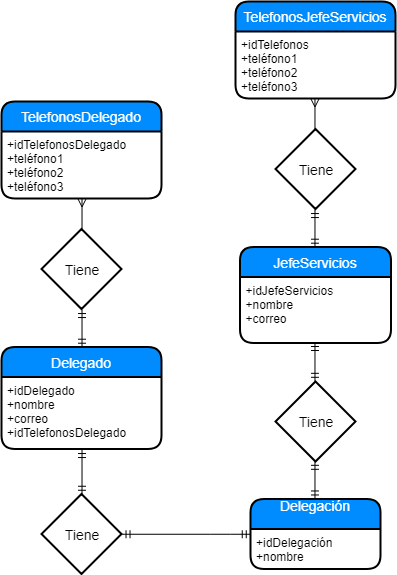
\includegraphics[width=.60\textwidth]{images/capitulo3/ModeloDominio.png}
		\caption{Modelo de dominio de programa}
		\label{InfoyDatos:ModeloDominio}
	\end{center}
\end{figure}
\clearpage
%\subsubsection{Interacción con el usuario}
\begin{itemize}
    \item La aplicación debe ser amigable con el usuario al momento de la interacción entre usuario y sistema.
    \item Responsive, es decir, que sea visualizable en la mayoria de los dispositivos.
\end{itemize}
%\hypertarget{BR:BR1}{}
\begin{BussinesRule}{BR1}{Precio de Espectaculares}%%%Redactado por Montiel Guerrero Christian Omar
    \BRitem[Tipo: ] Habilitadora
    \BRitem[Clase:] Condicional
    \BRitem[Nivel:] Influencia de precios
    \BRitem[Descripción:] El Gerente de Infraestructura determinara los precios de los espectaculares de acuerdo a su tamaño, tipo de espectacular y la vía en la que este localizada.
    \BRitem[Motivación: ] Un mejor control 
    a la hora de designar el precio a los espectaculares
    \BRitem[Ejemplo positivo: ] El Gerente de Infraestructura cuenta con la información del tamaño del espectacular, su tipo y la vía en la que se encuentra.
    \BRitem[Ejemplo negativo: ] El Gerente de Infraestructura no cuenta con dicha información antes mencionada, por lo que tiene que designar el precio, puede que el precio sea erróneo.
\end{BussinesRule}

\hypertarget{BR:BR2}{}
\begin{BussinesRule}{BR2}{Notificación de estado de espectacular}
%AngelDLR
    \BRitem[Tipo: ] Regla de inferencia de un hecho.
    \BRitem[Clase:] Habilitadora
    \BRitem[Nivel:] Control
    \BRitem[Descripción:] Se determina el estado de un espectacular seleccionado y con base en eso se notifica al personal de la empresa que necesite conocer el estado de un espectacular.Lo estados pueden ser:
    \begin{itemize}
        \item Disponible
        \item En mantenimiento
        \item No disponible
        \item Dado de baja
        \item En reparación
        \item Con incidente
    \end{itemize}
    \BRitem[Motivación:] Llevar un correcto control del estado en el que se encuentran los espectaculares ayudara a optimizar los tiempos de trabajo de las tareas relacionadas a los estados de los espectaculares. 
   % \BRitem[Sentencia:] 
    %\if estado = "Disponible" \bigwedge notificación = "Espectacular disponible"
    %\if estado = "En mantenimiento" \bigwedge notificación = "Espectacular en mantenimiento"
    \BRitem[Motivación:] Dar atención rápida a los problemas que se puedan generar por el desconocimiento de los espectaculares.
    \BRitem[Ejemplo positivo:] {\em Estado de espectacular:}En mantenimiento
    \BRitem[Ejemplo negativo:] {\em Estado de espectacular:}Desconocido
\end{BussinesRule}

\hypertarget{BR:BR3}{}
\begin{BussinesRule}{BR3}{Emisión de un oficio para un permiso legal}
    \BRitem[Tipo: ] Ejecutivo
    \BRitem[Clase:] Integridad
    \BRitem[Nivel:] Pendiente
    \BRitem[Descripción:] Los permisos legales se solicitan al gobierno mediante un oficio en donde se redacta cuáles espectaculares se solicita utilizar como espacios publicitarios. Un oficio tiene un folio de control expedido por el gobierno.
    \BRitem[Motivación:] Mantener el control de cuáles espectaculares fueron autorizados para utilizarse con fines publicitarios.
\end{BussinesRule}

% Regla de negocio basado en https://www.gob.mx/tramites/ficha/permiso-de-instalacion-de-anuncios-publicitarios/SCT949
% CONAR, http://www.conar.org.mx/que_es_conar
\hypertarget{BR:BR4}{}
\begin{BussinesRule}{BR4}{Modificación del estado de un permiso legal}
    \BRitem[Tipo: ] Habilitadora
    \BRitem[Clase:] Restricción
    \BRitem[Nivel:] Control
    \BRitem[Descripción:] Los permisos legales para hacer uso de los espacios físicos en la vía publica requieren de un permiso emitido por la Secretaría de Comunicaciones y Transportes. Esta dependencia del gobierno es la que determina todas las solicitudes de permisos y los cambios que puedan existir en ellos.
    
    \BRitem[Motivación: ] Mantener un negocio funcionando de acuerdo a las leyes y normas que establece el gobierno de las zonas en donde se ubican los espacios publicitarios. Como consecuencia, el gobierno puede determinar el estado del permiso de los espectaculares considerados dentro del negocio como:
    \begin{itemize}
        \item Vigente
        \item En trámite
        \item Vencido
    \end{itemize}
    \BRitem[Ejemplo positivo: ] Estado del permiso de un espectacular: vigente.
    \BRitem[Ejemplo negativo: ] Estado del permiso de un espectacular: vencido.
\end{BussinesRule}

\hypertarget{BR:BR5}{}
\begin{BussinesRule}{BR5}{Periodo de vigencia del permiso legal}
    \BRitem[Tipo: ] Ejecutiva
    \BRitem[Clase:] Restricción
    \BRitem[Nivel:] Control
    \BRitem[Descripción:] Por políticas de la empresa, los espectaculares con permisos vencidos no pueden considerarse dentro de las posibles soluciones publicitarias. Por lo tanto, un agente de venta no tiene autorización para proponerla a un cliente.
    
    \BRitem[Motivación: ] Mantener la satisfacción de los clientes, respetando el acuerdo inicial dentro del contrato evitando contratiempos y acciones que no fueron consideradas para mantener el proyecto publicitario.
\end{BussinesRule}

\hypertarget{BR:BR6}{}
\begin{BussinesRule}{BR6}{Acceso a la información de solo los clientes asignados}
    \BRitem[Tipo: ] Habilitadora
    \BRitem[Clase:] Autorización
    \BRitem[Nivel:] Control
    \BRitem[Descripción:] Un agente de ventas puede ver la información únicamente de los clientes que se le han asignado.
    \BRitem[Motivación:]Llevar un control sobre que agente de ventas lleva la información de cada uno de los clientes y evitar que alguien haga mal uso de esta.
    \BRitem[Ejemplo positivo:] Solo el agente de ventas asignado y el gerente de ventas pueden tener acceso a la información de los clientes. 
    \BRitem[Ejemplo negativo: ] Un agente de ventas no asignado a esos clientes tenga acceso a información que no le corresponde. 
\end{BussinesRule}

%Regla redactada por Karla 
\hypertarget{BR:BR7}{}
\begin{BussinesRule}{BR7}{Incumplimiento de contrato}
    \BRitem[Tipo: ] Habilitadora
    \BRitem[Clase:] Condicional
    \BRitem[Nivel:] Control
    \BRitem[Descripción:] Si el cliente o la empresa no pueden cumplir con lo definido en el contrato que firmaron por común acuerdo, el que incumpla con dicho documento sera acreedor a una sanción. Se deberá pagar la pena convenida en el contrato.
    \BRitem[Motivación: ] Saber que hacer en caso de que alguna de las partes involucradas en el contrato(la empresa o el cliente) incumpla con las obligaciones, términos y condiciones que fueron pactadas por común acuerdo.
    \BRitem[Ejemplo positivo:] La sanción o pena pactada sea pagada, sin ninguna oposición de alguna de las dos partes. 
    \BRitem[Ejemplo negativo: ] Que alguna de las dos partes no quisiera hacerse responsable y pagar la sanción que le corresponde.
\end{BussinesRule}

%Regla redactada por Karla 
\hypertarget{BR:BR8}{}
\begin{BussinesRule}{BR8}{Atención de ciertos vendedores dependiendo de la dirección del cliente}
    \BRitem[Tipo: ] Habilitadora
    \BRitem[Clase:] Restricción
    \BRitem[Nivel:] Control
    \BRitem[Descripción:]Dependiendo de la delegación en donde residan los clientes sera el agente de ventas que los atenderá, con esto se quiere dar a entender que los agentes de ventas de la empresa se dividirán en grupos y cada uno de estos atenderá una delegación distinta, por ejemplo, que  los clientes cuyo domicilio se encuentre en la delegación Gustavo A. Madero no podrán ser atendidos por vendedores que atienden a la Delegación Cuauhtémoc o Alvaro Obregón.
  
    \BRitem[Motivación: ]Brindar un mejor y mas ágil servicio a los clientes, ya que esto permitirá que tanto el vendedor como el cliente puedan desplazarse mas fácilmente para establecer los términos del contrato y además ayudara a la empresa a tener un mayor control y administración sobre los clientes que se están llevando en cada zona. 
    \BRitem[Ejemplo positivo:] Los clientes al ser atendidos por vendedores cercanos a la zona en donde residen , tienen una mejor comunicación con ellos.
    \BRitem[Ejemplo negativo: ] Los vendedores llegan a ser insuficientes o excesivos para determinada zona.
\end{BussinesRule}

%Regla redactada por Karla
\hypertarget{BR:BR9}{}
\begin{BussinesRule}{BR9}{Espectaculares en Funcionamiento}
    \BRitem[Tipo: ] Habilitadora
    \BRitem[Clase:] Condicional
    \BRitem[Nivel:] Control
    \BRitem[Descripción:]El agente de ventas sólo podrá ofrecer a sus clientes espectaculares en renta que estén funcionando correctamente, es decir, que no tengan ningún fallo o se encuentren en reparación. Si no es así, entonces los agentes de ventas no podrán ofrecerlos. 
    \BRitem[Motivación:] Brindar un servicio de alta calidad,garantizando a los clientes que sus espectaculares le serán entregados en buenas condiciones.
    \BRitem[Ejemplo positivo:]Los espectaculares rentados no presentan ninguna falla
    \BRitem[Ejemplo negativo:] Los espectaculares presentan alguna falla en los primeros días de ser rentados
\end{BussinesRule}

\hypertarget{BR:BR10}{}
\begin{BussinesRule}{BR10}{Retraso en el servicio de instalación de publicidad}%%Redactado por Alberto Franco 
    \BRitem[Tipo: ] Ejecutivo
    \BRitem[Clase:] Condición 
    \BRitem[Nivel:] Control
    \BRitem[Descripción:] El gerente de personal de instalación y mantenimiento asignara nuevo personal para la instalación lo mas pronto posible en el servicio de instalación de un ser vicio de publicidad 
    \BRitem[Motivación: ] evitar retrasos en los servicios, evitando la perdida de clientes o un servicio insatisfactorio por parte del cliente
    \BRitem[Ejemplo positivo: ] Los espectaculares de un servicio se instalan correctamente (a tiempo y en forma)
    \BRitem[Ejemplo negativo: ] Existe un retraso en la instalación de espectaculares de un servicio y a cliente le urge
\end{BussinesRule}

\hypertarget{BR:BR11}{}
\begin{BussinesRule}{BR11}{Adición de nuevos espectaculares al contrato}
%Regla redactada por Edgar Roa
    \BRitem[Tipo: ] Regla de integridad referencial.
    \BRitem[Clase:] Cronometrada.
    \BRitem[Nivel:] Control.
    \BRitem[Descripción: ] Si el cliente solicita más espectaculares para su compaña publicitaria se creará un nuevo contrato.
    \BRitem[Motivación: ] Evitar trámites con la Secretaría de Hacienda y Crédito Público.
    \BRitem[Sentencia: ] $ if(tiempoDeContrato \hspace{0.1cm} \geq \hspace{0.1cm} 30 dias) \Rightarrow generarContrato() $.
    \BRitem[Ejemplo positivo:]
    \begin{itemize}
        \item Se agregó 1 espectacular al contrato.
        \item Se agregaron 4 espectaculares al contrato.
        \item Se agregaron 9 espectaculares al contrato.
    \end{itemize}
    \BRitem[Ejemplo negativo:]
    \begin{itemize}
        \item Se agregaron 0 espectaculares al contrato.
        \item No se pudo agregar 2 espectaculares al contrato.
    \end{itemize}
\end{BussinesRule}


\hypertarget{BR:BR12}{}
\begin{BussinesRule}{BR12}{Eliminación de espectaculares}
%Regla redactada por Edgar Roa
    \BRitem[Tipo: ] Regla de integridad referencial.
    \BRitem[Clase:] Restricción.
    \BRitem[Nivel:] Control.
    \BRitem[Descripción: ] Si se requiere eliminar un espectacular se podrá dar de baja o eliminarse definitivamente, siempre y cuando no existan contratos asociados.
    \BRitem[Motivación: ] Eliminar espectaculares dados de alta de manera accidental o darlos de baja para no mostrarlos disponibles.
    \BRitem[Sentencia: ] $ if(!existeContrato() \Rightarrow darDeBajaEspectacular() \hspace{0.2cm} || \hspace{0.2cm} eliminarEspectacularDefinitivamente() $.
\end{BussinesRule}
%Regla redactada por Edgar Roa
%Caso de uso
%\begin{BussinesRule}{BR12}{Notificación de vencimiento de permiso legal}
%    \BRitem[Tipo: ] Regla de inferencia de un hecho.
%    \BRitem[Clase:] Cronometrada.
%    \BRitem[Nivel:] Influencia.
%    \BRitem[Descripción: ] El cliente recibirá 1 notificación cada 3 días a partir de los últimos 15 días de vencimiento del contrato. El contrato podrá ser renovado con la opción de mantener el contrato con las mismas especificaciones que el anterior o hacer un nuevo contrato.
%    \BRitem[Motivación: ] Preguntar al cliente si desea renovar el contrato.
%    \BRitem[Sentencia: ] $ if(existeContrato \hspace{0.1cm} \land \hspace{0.1cm} fechaDeTerminoDeContrato \hspace{0.1cm} \geq \hspace{0.1cm} 15 días \hspace{0.2cm} NotificarVencimientoDeContrato()$.
%\end{BussinesRule}

\hypertarget{BR:BR13}{}
\begin{BussinesRule}{BR13}{Notificación de renovación de seguro de espectaculares}
%Angel DLR
%Caso de uso
    \BRitem[Tipo:] Regla de integridad estructural.
    \BRitem[Clase:] Ejecutiva
    \BRitem[Nivel:] Control
    \BRitem[Descripción:] El departamento jurídico recibe una notificación que le permite conocer que seguros de espectaculares están próximos a vencer.
    \BRitem[Motivación:] Se requiere que los espectaculares estén protegidos ante los diferentes incidentes que puedan ocurrir, y así evitar perdidas monetarias a la empresa.
    \BRitem[Sentencia:] $ if \hspace{0.2cm} fechaDeVencimientoSeguro <= 20 días \hspace{0.2cm} \Rightarrow  Notificación de Renovación de Seguro $. 
    \BRitem[Ejemplo positivo:] Quedan 20 días para renovar la póliza de seguro con el número SE-123
    \BRitem[Ejemplo negativo:] Sin notificación de renovación de póliza de seguro, en los veinte días anteriores a la fecha de vencimiento de la póliza de seguro.
\end{BussinesRule}

\hypertarget{BR:BR14}{}
\begin{BussinesRule}{BR14}{Categorización de espectaculares por tamaño}
%Angel DLR
     \BRitem[Tipo:] Regla de operación.
    \BRitem[Clase:] Ejecutiva
    \BRitem[Nivel:] Control
    \BRitem[Descripción:] Categorizar el espectacular de acuerdo a su tamaño.
    \BRitem[Motivación:] Se requiere tener los espectaculares distribuidos en tres categorías de acuerdo a su tamaño, es decir: Grande, Mediano y Chico. 
    \BRitem[Sentencia:] \hspace{0.2cm}\\
        $ if  \hspace{0.2cm} medidaEspectacular < 25 m^2 \hspace{0.2cm} \Rightarrow Tamaño = Chico $.\\ 
        $ if  \hspace{0.2cm} medidaEspectacular > 25 m^2 \bigwedge \hspace{0.2cm} medidaEspectacular < 80 m^2 \hspace{0.2cm} \Rightarrow Tamaño = Mediano $.\\
        $ if  \hspace{0.2cm} medidaEspectacular > 80 m^2 \hspace{0.2cm} \hspace{0.2cm} \Rightarrow Tamaño = Grande $.\\
    %\BRitem[Ejemplo positivo:] 
    %\BRitem[Ejemplo negativo:] 
\end{BussinesRule}

%\begin{BussinesRule}{BR15}{Notificación de adquisición de nuevo espectacular}%%%Redactado por Alberto Franco
%    \BRitem[Tipo: ] Pendiente
%    \BRitem[Clase:] Pendiente
%    \BRitem[Nivel:] Influencia
%    \BRitem[Descripción:] El gerente de infraestructura notificara cuando se ha adquirido un nuevo espectacular y ya está listo (contando con todas las especificaciones, como son permiso, haber tenido un mantenimiento preventivo etc) para poder hacer uso de dicho espectacular.
%    \BRitem[Motivación: ] Un mejor control cuando hay adquisiciones de espectaculares, beneficiando al agente de ventas.
%    \BRitem[Ejemplo positivo: ] El agente de ventas cuenta con la información actualizada constantemente de cada espectacular nuevo y disponible para usar y lo contempla al momento de ofrecérselo a un cliente
%    \BRitem[Ejemplo negativo: ] EL agente de ventas no cuenta con dicha información antes mencionada, por lo tanto no tiene una amplia gama de posibilidades de ofrecerle otros espectaculares a un cliente cuando el espectacular que tenia contemplado no esta disponible para poderlo rentar 
%\end{BussinesRule}
\hypertarget{BR:BR15}{}
\begin{BussinesRule}{BR15}{Contratación de Espectacular}%%%Redactado por Montiel Guerrero Christian Omar
    \BRitem[Tipo: ] Habilitadora
    \BRitem[Clase:] Condicional
    \BRitem[Nivel:] Control
    \BRitem[Descripción:] Cualquiera que requiera acceder al sistema deberá de tener un correo y una contraseña dentro del sistema.
    \BRitem[Motivación: ] Que ninguna persona ajena a la empresa a excepción de los clientes puedan acceder a la información confidencial.
\end{BussinesRule}

\hypertarget{BR:BR16}{}
\begin{BussinesRule}{BR16}{Inicio de sesión}%%%Redactado por Edgar Roa
    \BRitem[Tipo: ] Habilitadora
    \BRitem[Clase:] Condicional
    \BRitem[Nivel:] Influencia
    \BRitem[Descripción:] Cada espectacular contratado debe contratarse por lo menos por 30 días.
    \BRitem[Motivación: ] Que el cliente en esos 30 días verifique que nuestro servicio es de calidad.
\end{BussinesRule}

\hypertarget{BR:BR17}{}
\begin{BussinesRule}{BR17}{Dimensiones de un espectacular}%%%Redactado por Edgar Roa
    \BRitem[Tipo: ] Habilitadora
    \BRitem[Clase:] Condicional
    \BRitem[Nivel:] Influencia
    \BRitem[Descripción:] Cada espectacular debe contar con un ancho y alto mínimo de 2 mtrs.
    \BRitem[Motivación: ] Brindar espacios publicitarios de tamaño accesible y visible al público.
\end{BussinesRule}

\clearpage
%\hypertarget{cap:infoydats}{}
\subsubsection{Información y datos}
\textbf{Modelo de dominio - Delegación}
Dentro del siguiente modelo de datos se presenta un prototipo en modelo Entidad-Relación de la delegación.

\begin{figure}[htbp!]
	\begin{center}
	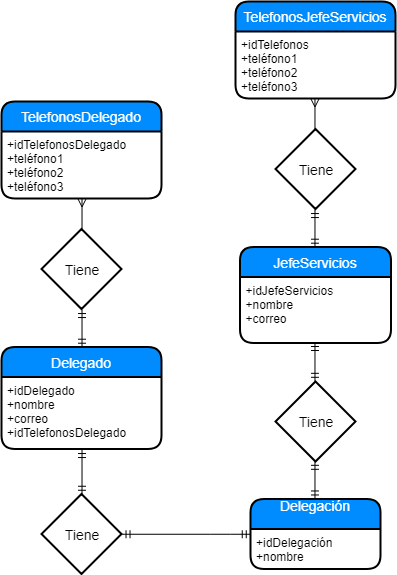
\includegraphics[width=.60\textwidth]{images/capitulo3/ModeloDominio.png}
		\caption{Modelo de dominio de programa}
		\label{InfoyDatos:ModeloDominio}
	\end{center}
\end{figure}
\clearpage
%\subsubsection{Propiedades del software}
\begin{itemize}
    \item El software debe ser amigable con el cliente y los empleados que lo utilicen.
\item\textbf{Seguridad:} El usuario deberá proporcionar su nombre de usuario y contraseña para acceder al sistema.
\item\textbf{Usabilidad:} Nuestra meta es que todos los usuarios que utilicen el sistema aprendan a utilizarlo de forma correcta, así mismo que al menos el 95 por siento comprendan los resultados que se pueden obtener al utilizarlo. 
     \item \textbf{Eficiente:} El software debe ser eficiente, para esto se deben
cumplir las 3 subpropiedades: funcionalidad, tiempo de respuesta y utilización mınima de recursos.

\textbf{Eficiencia en tiempo de respuesta:}
Cuando el usuario realice una petición al sistema o seleccione una acción, nuestra meta es que el tiempo de respuesta (medido en segundos)  sea menor o igual a 5. 

\textbf{Funcionalidad:}
Se refiere a la capacidad de realizar el trabajo designado. 
Para comprobar si nuestro sistema es eficiente en funcionalidad,debemos de realizar una serie de pruebas basadas en los requerimientos funcionales que definimos con anterioridad y observar el funcionamiento del sistema.
 \item
\textbf{Atractivo} El software debe ser atractivo para el usuario.Para esto debemos acudir con el cliente y presentarle las diferentes opciones
acerca del diseño visual del sistema y compartir opiniones para llegar a un acuerdo y  desarrollar la versión final del
producto.
\item\textbf{Modificable:} Nuestra meta es que el sistema sea capaz de adoptar cualquier tipo de modificación o extensión de un modulo sin
dejar inservible algún otro. Para esto planeamos tomar el tiempo requerido para implementar una modificación en el sistema,
dicha modificación deberá incluir diseño, implementación y modificación de los cambios realizados.
\end{itemize}
\clearpage
%\section{Modelado de procesos}
\input{proc/proc01.tex}
%%=========================================================
\chapter{Modelo dinámico}
\label{cap:ModeloDinamico}

Este capítulo describe en modelo dinámico del sistema. en el se detallan todos los escenarios de ejecución del sistema asi como el comportamiento que tendra el sistema a lo largo de tiempo se uso.
%---------------------------------------------------------
%\section{Maquina de estados}

%---------------------------------------------------------
\clearpage
\section{Modelo de Maquinas de Estado}
\begin{figure}[htbp!]
    \centering
    \includegraphics[width=0.8\textwidth]{Capitulo4/edo_especta.jpg}
    \caption{Diagrama de estados del estatus de espectacular}
    \label{fig:my_label}
\end{figure}
\textbf{ins-estru:} el estatus del espectacular pasa a \textbf{Disponible} cuando se hace la instalación exitosa de la estructura del espectacular.
\\
\textbf{inic[contrato]:} Cuando el PIMDE hace la instalación de la lona espectacular, el estatus pasa a \textbf{No disponible} cuando hay un contrato. 
\\
\textbf{fin[Contrato]:} cuando se acaba el contrato de la renta de la estructura del espectacular, el estatus pasa a \textbf{Disponible}.
\\
\textbf{fecha-progra:} el estatus del espectacular pasa a \textbf{En mantenimiento} cuando la fecha programada para su mantenimiento esta próxima.
\\
\textbf{reg-positivo:} El estatus del espectacular pasa a \textbf{No disponible} o \textbf{Disponible} cuando hay un registro positivo del mantenimiento del mismo.
\\
\textbf{reg-negativo:} cuando hay un registro negativo del mantenimiento del espectacular se queda ahí mismo.
\textbf{inst-defe} Al momento de hacer un mantenimiento del espectacular y el PIMDE se percata que la estructura no soporta otro mantenimiento ya sea correctivo o preventivo, notifica al Gerente de Infraestructura para que cambie el estatus a \textbf{Baja}
\textbf{term[Contrato]:} Cuando se termina el contrato de renta de espacio con el arrendatario cambia el estatus del espectacular a \textbf{Baja}
\clearpage

\begin{figure}[htbp!]
    \centering
    \includegraphics[width=0.8\textwidth]{Capitulo4/edo_servicio.jpg}
    \caption{Diagrama de estados del estatus del servicio}
    \label{fig:my_label}
\end{figure}
\textbf{ini-esta:} 
el estatus del servicio que se realiza en la estructura del espectacular por defecto se encuentra en \textbf{No realizado}.
\\
\textbf{asig-serv:}
el estatus de la estructura del espectacular pasa a \textbf{En proceso}, cuando el Gerente de Infraestructura asigna al PIMDE un servicio y este se encuentra en el lugar en donde se tiene que realizar el servicio.
\\
\textbf{si\_Realizado:}
el estatus de la estructura del espectacular pasa a \textbf{Realizado}, cuando el PIMDE realizó un servicio exitoso sobre la estructura del espectacular.
\\
\textbf{no\_Realizado:}
el estatus de la estructura del espectacular pasa a \textbf{No realizado}, cuando el PIMDE no pudo realizar un servicio exitoso sobre la estructura del espectacular.
\clearpage

\section{Modelo de Casos de Uso}

\begin{figure}[htbp!]
    \centering
    \includegraphics[angle=90, width=0.80\textwidth]{Capitulo4/ModeloGeneralCU.jpg}
    \caption{Diagrama General de Casos de uso}
    \label{fig:my_label}
\end{figure}

% CASOS DE USO
\input{cu/CU00}
\input{cu/CU01}
\input{cu/CU02}
\input{cu/CU03}
\input{cu/CU04}
\input{cu/CU05}
\input{cu/CU06}
\input{cu/CU07}
%\input{cu/CU08}
%\input{cu/CU09}
%\input{cu/CU10}
\input{cu/CU11}
\input{cu/CU12}
\input{cu/CU13}
\input{cu/CU14}
\input{cu/CU15}
\input{cu/CU16}
%\input{cu/CU17}
%\input{cu/CU18}
%\input{cu/CU19}
%\input{cu/CU20}
\input{cu/CU21}
\input{cu/CU22}
%%=========================================================
\chapter{Modelo de la interacción}	
\label{cap:ModeloDeLaInteraccion}
    En este capítulo se describen gráficamente la estructura de la interfaz gráfica diseñadas para cubrir las necesidades de los usuarios objetivos de acuerdo a los modelos definidos anteriormente.
\section{Modelo de navegación}
\clearpage
\section{Interfaces de Aplicación}

\subsection{Home}
\hypertarget{IU:IU-HOME}{}
    Página principal, con barra de menú de servicios proporcionados por la empresa y botón de inicio de sesión.
Dentro del Home se muestran las opciones
\begin{itemize}
    \item Inicio
    \item ¿Quienes Somos?
         \\Descripción de la empresa,misión y visión.
    \item Servicios Adicionales
         \\Opciones que ofrece la empresa para su publicidad.
    \item Registrarme para Cotizar
         \\Registro abierto para los clientes.
    \item Contactanos
        \\Datos de la empresa.
\end{itemize}
\begin{figure}[htbp!]
    \centering
    \includegraphics[width=1.0\textwidth]{images/Capitulo3/IU-00.png}
    \caption{Home de la Página}
    \label{fig:my_label}
\end{figure}
\clearpage

\hypertarget{IU:IU-Login}{}
\subsection{IU-Login}
    Pantalla que permite al usuario iniciar sesión dentro del sistema.
\begin{itemize}
    \item Correo electrónico.Campo alfanumérico.(Obligatorio)
    \item Contraseña.Campo alfanumérico que será representado por asteriscos en pantalla.(Obligatorio)
\end{itemize}
\begin{figure}[htbp!]
    \includegraphics[width=1.0\textwidth]{images/Capitulo3/IU-C-Login.jpg}
    \caption{Inicio de Sesión}
    \label{fig:my_label}
\end{figure}
\clearpage

\hypertarget{IU:IU-CC}{}
\subsection{IU-CC}
    Pantalla que permite al usuario hacer el cambio de su contraseña.
\begin{itemize}
    \item Contraseña.Campo alfanumérico que será representado por asteriscos en pantalla.(Obligatorio)
\end{itemize}
\begin{figure}[htbp!]
    \includegraphics[width=1.0\textwidth]{images/Capitulo3/IU-01.jpg}
    \caption{Cambio de Contraseña}
    \label{fig:my_label}
\end{figure}
\clearpage

\hypertarget{IU:IU-RC}{}
\subsection{IU-RC}
   Pantalla que permite al cliente la recuperación de su contraseña.
    \begin{itemize}
        \item Correo electrónico. 
    \end{itemize}
\begin{figure}[htbp!]
    \includegraphics[width=1.0\textwidth]{images/Capitulo3/IU-08.jpg}
    \caption{Recuperación de cuenta}
    \label{fig:my_label}
\end{figure}
\clearpage

\hypertarget{IU:IU-GI-Login}{}
\subsection{IU-GI-Login}
    Pantalla de acceso del Gerente de Infraestructura.
\begin{figure}[htbp!]
    \includegraphics[width=1.0\textwidth]{images/Capitulo3/IU-GI.jpg}
    \caption{Menú de opciones desde el perfil del Gerente de Infraestructura}
    \label{fig:my_label}
\end{figure}
\clearpage


\hypertarget{IU:IU-REG}{}
\subsection{IU-REG}
    Pantalla de registro de cliente para poder obtener usuario y contraseña.
\begin{itemize}
    \item Tipo de Persona. Campo en lista desplegable con los valores Física y Moral.(Obligatorio)
    \item RFC. Campo alfanumérico.(Obligatorio)
    \item Nombre o Razón Social. Campo alfanumérico.(Obligatorio)
    \item Apellido Paterno. Campo alfanúmerico.
    \item Apellido Materno. Campo alfanúmerico.
    \item Correo electrónico. Campo alfanumérico. (Obligatorio)
    \item Teléfono. Campo numérico. (Obligatorio)
    \item Password. Campo alfanúmerico.(Obligatorio)
    \item Calle. Campo alfanumérico. (Obligatorio)
    \item Colonia. Campo alfanumérico.(Obligatorio)
    \item Código Postal.Campo numérico.(Obligatorio)
    \item Delegación o Municipio. Campo autocompletable en lista despegable. (Obligatorio) 
    \item Estado. Campo en lista desplegable con los valores:Ciudad de México y Estado de México.(Obligatorio)
    \item Checkbox de Términos y Condiciones.(Obligatorio)
    \item Captcha.
\end{itemize}
\begin{figure}[htbp!]
    \centering
    \includegraphics[width=0.85\textwidth]{images/Capitulo3/IU-C-Register.jpg}
    \caption{Registro del Cliente}
    \label{fig:my_label}
\end{figure}
\clearpage

\hypertarget{IU:IU-GI-AE}{}
\subsection{IU-GI-AE}
    Capturar en sistema las características de un nuevo espectacular para su posterior venta.
    \begin{itemize}
    \item ID Espectacular. Campo capturado automatico.
    \item Estado. Campo en lista desplegable con las opciones: Disponible, No disponible, En Mantenimiento, Dado de Baja.
    \item Tipo de Espectacular. Campo en lista despegable con las opciones Iluminado, Dos Caras, MonoPoste, Tres Caras.
    \item Vía. Campo en lista despegable con las opciones Primaria, Secundaria y VIP.
    \item Precio. Campo númerico.
    \item Imagen. Formato JPG
    \item Ancho. Campo númerico.
    \item Alto. Campo númerico.
    \item Nombre de Contacto. Campo alfanúmerico.
    \item CURP. Campo alfanúmerico.
    \item Teléfono. Campo alfanúmerico.
    \item Dirección Arrendador.Campo alfanúmerico.
    \item RFC Arrendador.Campo alfanúmerico.
    \item Correo electrónico.Campo alfanúmerico.
    \item Dirección. Campo alfanúmerico.
    \item Colonia.Campo alfanúmerico.
    \item Delegación - Municipio. Campo en lista despegable con las siguientes opciones.
    \begin{enumerate}
        \item Álvaro Obregón.
        \item Benito Juárez.
        \item Coyoacán.
        \item Cuajimalpa.
        \item Cuauhtémoc.
        \item Gustavo A. Madero.
        \item Iztacalco.
        \item Magdalena Contreras.
        \item Iztapalapa
    \end{enumerate}
    \end{itemize}
\begin{figure}[htbp!]
    \includegraphics[width=0.9\textwidth]{images/Capitulo3/IU-GI-RegEsp.jpg}
    \caption{ Alta un Espectacular}
    \label{fig:my_label}
\end{figure}
\clearpage


\subsection{IU-GI-CE}
    Consulta de Espectaculares
\begin{itemize}
    \item Muestra los espectaculares dados de alta en sistema mediante un mapa de google maps.
    \item Delegación.Campo en lista desplegable con las opciones
    \begin{enumerate}
        \item Álvaro Obregón.
        \item Benito Juárez.
        \item Coyoacán.
        \item Cuajimalpa.
        \item Cuauhtémoc.
        \item Gustavo A. Madero.
        \item Iztacalco.
        \item Magdalena Contreras.
        \item Iztapalapa
    \end{enumerate}
    \item Zona. Campo en lista despegable con las opciones Norte, Sur, Centro, Poniente y Oriente.
    \item Vía. Campo en lista despegable con las opciones Primaria, Secundaria y VIP.
    \item Tipo.Campo en lista despegable con las opciones Simple, Doble, Triple,Digital y Dinámico.
    \item Tamaño. Campo en lista despegable con opciones Chico, Mediano y Grande.
    \item Estado. Campo en lista despegable con las opciones Disponible, No Disponible,En mantenimiento y Dado de Baja.
    
\end{itemize}
\begin{figure}[htbp!]
    \centering
    \includegraphics[width=0.95\textwidth]{images/Capitulo3/IU-GI-CE.jpg}
    \caption{Pantalla para consulta de espectaculares}
    \label{fig:my_label}
\end{figure}
\clearpage

\subsection{IU-GI-NPIMDE}
    Gerente de Infraestructura  recibe una notificación de una nueva solicitud de servicio, el Gerente de Infraestructura selecciona la notificación que desea asignar.
    \begin{figure}[htbp!]
    \centering
    \includegraphics[width=1.0\textwidth]{images/Capitulo3/IU-6.jpg}
    \caption{Notificación Gerente de Infraestructura}
    \label{fig:my_label}
\end{figure}
\clearpage

\subsection{IU-GI-APIMDE}
    Asignación de tareas a PIMDE.
    Detalles del servicio solicitado en columna de lado izquierdo, con las características del espectacular, del lado derecho filtros de búsqueda por:
    \begin{itemize}
        \item ID PIMDE
        \item Nombre del empleado
    \end{itemize}
     Ingreso de la Fecha de asignación de tarea.
\begin{figure}[htbp!]
    \centering
    \includegraphics[width=0.9\textwidth]{images/Capitulo3/IU-7.jpg}
    \caption{Asignación de PIMDE a un nuevo  servicio.}
    \label{fig:my_label}
\end{figure}
\clearpage

\subsection{IU-AV-Cot}
    Pantalla de Cotización de Espectaculares.
    \begin{itemize}
    \item Tipo de Campaña. Campo en lista desplegable.
    \item Tipo de Espectacular. Campo en lista desplegable.
    \item Vía.Campo en lista desplegable con las opciones Vía Primaria, Secundaria y VIP. 
    \item Zona Campo en lista desplegable
    \item Delegación. Campo en lista desplegable.
    \item Ancho
    \item Alto
    \item Precio
    \end{itemize}
\begin{figure}[htbp!]
    \centering
    \includegraphics[width=0.9\textwidth]{images/Capitulo3/IU-AV-Cot.jpg}
    \caption{Cotización de Espectaculares}
    \label{fig:my_label}
\end{figure}
\clearpage

%\hypertarget{IU:IU-AV-Login}{}
%\subsection{IU-AV-Login}
 %   La siguiente pantalla corresponde al inicio de sesión del agente de ventas.
    
%\begin{figure}[htbp!]
%    \centering
%    \includegraphics[width=0.9\textwidth]{images/Capitulo3/IU-AV-Login.png}
%    \caption{Login Agente de Ventas}
%    \label{fig:my_label}
%\end{figure}
%\clearpage

\hypertarget{IU:IU-AV-ConCli}{}
\subsection{IU-AV-ConCli}
    La siguiente pantalla es para visualizar la información del o los clientes que el agente de ventas necesite. Para ello cuenta con un buscador en el cuál puede ingresar el nombre del cliente y seleccionar en la parte izquierda de la lista desplegable ``Ver'' las clientes en grupos de 10 en 10 hasta 50 o todos los clientes con un nombre similar.
    
    Entre los campos que presenta para visualizar la información del cliente se encuentran:
    \begin{itemize}
        \item Nombre
        \item Apellido Paterno
        \item Apellido Materno
        \item Calle
        \item Delegación
        \item Cp
        \item Colonia
        \item Tipo de cliente
        \item Teléfono
        \item Email
    \end{itemize}
\begin{figure}[htbp!]
    \centering
    \includegraphics[width=0.9\textwidth]{images/Capitulo3/IU-AV-ConCli.png}
    \caption{Consultar clientes}
    \label{fig:my_label}
\end{figure}
\clearpage

\hypertarget{IU:IU-AV-ConEmp}{}
\subsection{IU-AV-ConEmp}
    La siguiente pantalla es para visualizar la información de una o varias empresas que el agente de ventas necesite. Para ello cuenta con un buscador en el cuál puede ingresar el nombre de la empresa y seleccionar en la parte izquierda de la lista desplegable ``Ver'' las empresas en grupos de 10 en 10 hasta 50 o todos los clientes con un nombre similar.
    
    Entre los campos que presenta para visualizar la información de las empresas se encuentran:
    \begin{itemize}
        \item Nombre o Razón social
        \item Tipo de cliente
        \item Teléfono
        \item Email
    \end{itemize}
\begin{figure}[htbp!]
    \centering
    \includegraphics[width=0.9\textwidth]{images/Capitulo3/IU-AV-ConEmp.png}
    \caption{Consultar empresas}
    \label{fig:my_label}
\end{figure}
\clearpage
\hypertarget{IU:IU-PIMDE-RG}{}
\subsection {IU:IU-PIMDE-RG}
Pantalla para capturar los servicios realizados por el PIMDE.
\begin{figure}[htbp!]
    \centering
    \includegraphics[width=0.9\textwidth]{images/Capitulo3/IU-15.jpg}
    \label{fig:my_label}
\end{figure}
\clearpage





%\hypertarget{IU-05-CambCon}{}
%\subsection{IU-05-CambCon}
%\begin{figure}[htbp!]
%    \centering
%    \includegraphics[width=0.9\textwidth]{images/Capitulo3/IU-14.png}
%    \caption{Cambio de contraseña}
%\end{figure}
%\clearpage%%

%%


%\subsection{IU-14}
%\begin{figure}[htbp!]
%    \centering
%    \includegraphics[width=0.9\textwidth]{images/Capitulo3/IU-14.png}
%    \caption{Registro Cliente}
%    \label{fig:my_label}
%\end{figure}
%\clearpage




%\subsection{UI-04-Form}
%    Pantalla de registro de Alta de Espectacular
%\begin{figure}[htbp!]
%\centering
%    \includegraphics[width=0.94\textwidth]{Capitulo4/C-U-02/2.png}
%    \caption{Formulario para Alta de Espectacular}
%    \label{fig:my_label}
%\end{figure}
%\subsection{UI-04-DatRegi}
%    Pantalla salida de Alta de Espectacular
%\begin{figure}[htbp!]
%\centering
%    \includegraphics[width=0.94\textwidth]{Capitulo4/C-U-02/3.png}
%    \caption{Formulario de salida de Alta de Espectacular}
%    \label{fig:my_label}
%\end{figure}
%\clearpage





\subsection{UI-01-PIMDE}
    Pantalla de inicio del usuario con el rol PIMDE
\begin{figure}[htbp!]
\centering
    \includegraphics[width=0.94\textwidth]{Capitulo4/C-U-08/1.png}
    \caption{Pantalla principal del PIMDE}
    \label{fig:my_label}
\end{figure}
\clearpage


\subsection{UI-02-PIMDEred}
    Pantalla de registro de trabajos realizados por parte del PIMDE
\begin{figure}[htbp!]
\centering
    \includegraphics[width=0.94\textwidth]{Capitulo4/C-U-08/2.png}
    \caption{Pantalla de registro de trabajos}
    \label{fig:my_label}
\end{figure}



\clearpage


\subsection{UI-03-PIMDEDatReg}
    Pantalla de registro exitoso del trabajo realizado por parte del PIMDE
\begin{figure}[htbp!]
\centering
    \includegraphics[width=0.94\textwidth]{Capitulo4/C-U-08/3.png}
    \caption{registro exitoso}
    \label{fig:my_label}
\end{figure}
\clearpage



%\subsection{UI-BS2LoginER}
%    Pantalla de inicio de sesión con un mensaje de error de que la contraseña es incorrecta de acuerdo al usuario
%\begin{figure}[htbp!]
%\centering
%    \includegraphics[width=0.94\textwidth]{ima%ges/Capitulo3/IU-11.jpg}
%    \caption{pantalla con error de contraseña}
%    \label{fig:my_label}
%\end{figure}
%\clearpage



%\subsection{UI-01-RecCon}
%    Pantalla de recuperación de contraseña del usuario, aquí se tiene que introducir el correo electrónico para que le sea proporcionada su contraseña.
%\begin{figure}[htbp!]
%\centering
%    \includegraphics[width=0.94\textwidth]{Capitulo4/C-U-10/2.png}
%    \caption{Pantalla de recuperación de contraseña}
%    \label{fig:my_label}
%\end{figure}
%\clearpage



\subsection{UI-02-CONSCOTI}
Pantalla de consulta de cotización de espectaculares, aquí el cliente podrá hacer una previa consulta de los espectaculares que necesite, con los datos que introduzca, podrá después ver el rango de precio que el pagara por esa renta
\begin{figure}[htbp!]
\centering
    \includegraphics[width=0.94\textwidth]{Capitulo4/C-U-20/DI-11.png}
    \caption{Formulario de cotización de espectaculares}
    \label{fig:my_label}
\end{figure}
\clearpage



\subsection{UI-03-msg}
En esta pantalla el cliente ya con su inicio de sesión previo y con el formulario lleno podrá saber la dirección de los espectaculares que solicito en el formulario así como también un rango de precio que el pagara antes de terminar el contrato.
\begin{figure}[htbp!]
\centering
    \includegraphics[width=0.94\textwidth]{Capitulo4/C-U-20/DI-12.png}
    \caption{Pantalla con la salida previa del precio que pagara el cliente}
    \label{fig:my_label}
\end{figure}
\clearpage


\hypertarget{IU:IU-C-Login}{}
\subsection{IU-C-Login}
Pantalla de inicio del usuario con el rol Cliente
\begin{figure}[htbp!]
\centering
    \includegraphics[width=0.94\textwidth]{Capitulo4/C-U-21/DI-13.png}
    \caption{Pantalla principal del Cliente}
    \label{fig:my_label}
\end{figure}
\clearpage



\subsection{UI-02-CLICONS}
En esta pantalla el cliente podrá hacer la consulta de espectaculares que tiene a su nombre, antes de meter algún filtro le aparecerán todos los espectaculares que están a su nombre.
\begin{figure}[htbp!]
\centering
    \includegraphics[width=0.94\textwidth]{Capitulo4/C-U-21/DI-14.png}
    \caption{Consulta de espectaculares general}
    \label{fig:my_label}
\end{figure}
\clearpage



\subsection{UI-02-CLICONS-1}
En está pantalla el cliente podrá hacer una consulta mas especifica de algún espectacular, insertando datos en los filtros de búsqueda.
\begin{figure}[htbp!]
\centering
    \includegraphics[width=0.94\textwidth]{Capitulo4/C-U-21/DI-15.png}
    \caption{Consulta de espectaculares especifico}
    \label{fig:my_label}
\end{figure}
\clearpage



\subsection{UI-01-CLI}
Pantalla de inicio del usuario con el rol Cliente
\begin{figure}[htbp!]
\centering
    \includegraphics[width=0.94\textwidth]{Capitulo4/C-U-23/DI-16.png}
    \caption{Pantalla principal del Cliente}
    \label{fig:my_label}
\end{figure}
\clearpage



\subsection{UI-02-CLIcap}
En esta pantalla ya con el id del espectacular que se le envía al cliente por correo electrónico por el cual no se tiene un pago reciente, el cliente lo inserta en el campo para poder efectuar el pago del espectacular.
\begin{figure}[htbp!]
\centering
    \includegraphics[width=0.94\textwidth]{Capitulo4/C-U-23/DI-17.png}
    \caption{Pago de espectacular}
    \label{fig:my_label}
\end{figure}
\clearpage



\subsection{UI-02-CLIcap2}
En esta pantalla al cliente se le notifica por medio de un mensaje que el pago fue cargado de manera exitosa.
\begin{figure}[htbp!]
\centering
    \includegraphics[width=0.94\textwidth]{Capitulo4/C-U-23/DI-18.png}
    \caption{Pago exitoso}
    \label{fig:my_label}
\end{figure}
\clearpage




\subsection{UI-01-AgeServ}
Pantalla de inicio del usuario con el rol Agente de Ventas
\begin{figure}[htbp!]
\centering
    \includegraphics[width=0.94\textwidth]{Capitulo4/C-U-25/DI-19.png}
    \caption{Pantalla principal del Agente de Ventas}
    \label{fig:my_label}
\end{figure}
\clearpage



\subsection{UI-02-REGISINCI}
Pantalla para registrar las incidencias que se han sucitado con los espectaculares, aquí el Agente de Ventas llena todos los campos para hacer un registro exitoso del incente.
\begin{figure}[htbp!]
\centering
    \includegraphics[width=0.94\textwidth]{Capitulo4/C-U-25/DI-19-0.png}
    \caption{Pantalla de registro de incidencias}
    \label{fig:my_label}
\end{figure}
\clearpage





\subsection{UI-03-RegiExit}
En esta pantalla el registro del incidente fue exitoso por lo cual este registro se manda al historial de incidentes que se han suscitado con ese espectacular
\begin{figure}[htbp!]
\centering
    \includegraphics[width=0.94\textwidth]{Capitulo4/C-U-25/DI-20.png}
    \caption{Registro exitoso de incidente}
    \label{fig:my_label}
\end{figure}
\clearpage






\subsection{UI-01-PCH}
Pantalla de inicio del usuario con el rol Personal de Capital Humano.
\begin{figure}[htbp!]
\centering
    \includegraphics[width=0.94\textwidth]{Capitulo4/C-U-30/DI-21.png}
    \caption{Pantalla principal del Personal de Capital Humano}
    \label{fig:my_label}
\end{figure}
\clearpage




\subsection{UI-02-FormAlt}
En esta pantalla el Personal de Capital Humano puede dar de alta el nuevo personal que llega a la empresa, solo que tiene que tener todos los datos que se piden en la pantalla para que no haya errores al dar de alta el nuevo personal.
\begin{figure}[htbp!]
\centering
    \includegraphics[width=0.94\textwidth]{Capitulo4/C-U-30/DI-22.png}
    \caption{Formulario de Alta de Personal}
    \label{fig:my_label}
\end{figure}
\clearpage



\subsection{UI-03-RegExit}
En esta pantalla el Personal de Capital Humano ya haciendo un registro previo, se muestra el registro ya realizado en el sistema y reflejado en la base de datos.
\begin{figure}[htbp!]
\centering
    \includegraphics[width=0.94\textwidth]{Capitulo4/C-U-30/DI-23.png}
    \caption{}
    \label{fig:my_label}
\end{figure}
\clearpage











\subsection{UI-01-PJPER}
\hypertarget{UI:UI-01-PJPER}{}
\begin{figure}[htbp!]
    \centering
    \includegraphics[width=0.94\textwidth]{Capitulo4/C-U-28/UI_Perfil_perjur.png}
    \caption{Perfil de usuario personal jurídico.}
    \label{fig:UI-01-PERPJ}
\end{figure}
\textbf{Descripción:} Perfil de usuario del personal jurídico. Permite a los usuarios con el cargo de personal jurídico registrar los seguros adquiridos así como los diferentes permisos que los espectaculares requieren para poder ser usados en los servicios de publicidad ofrecidos por la empresa.
\clearpage

\subsection{UI-02-PJNSEG}
\hypertarget{UI:UI-02-PJNSEG}{}
\begin{figure}[htbp!]
    \centering
    \includegraphics[width=0.94\textwidth]{Capitulo4/C-U-28/UI_NSeguro.png}
    \caption{Pantalla de registro de seguros de espectaculares.}
    \label{fig:UI-02-Nseg}
\end{figure}
\textbf{Descripción:} Esta interfaz de usuario permite al personal jurídico ingresar los datos principales que el sistema requiere para para poder notificar sobre renovación de seguros de espectaculares.
\clearpage

\subsection{UI-03-PJAE}
\hypertarget{UI:UI-03-PJAE}{}
\begin{figure}[htbp!]
    \centering
    \includegraphics[width=0.94\textwidth]{Capitulo4/C-U-28/UI_AgrEsp.png}
    \caption{Ventana para agregar espectaculares}
    \label{fig:my_label}
\end{figure}
\textbf{Descripción:} Esta interfaz de usuario permite al personal jurídico agregar los espectaculares que cubrirá el seguro o permiso que sera registrado.
\clearpage

\subsection{UI-04-PJNPER}
\hypertarget{UI:UI-04-PJNPER}{UI-04-PJNPER}
\begin{figure}[htbp!]
    \centering
    \includegraphics[width=0.94\textwidth]{Capitulo4/C-U-28/UI_NPer.png}
    \caption{Pantalla de registro de permisos de espectaculares.}
    \label{fig:my_label}
\end{figure}
Esta interfaz de usuario permite al personal jurídico ingresar los datos principales que el sistema requiere para para poder notificar sobre renovación de permisos de espectaculares.
\clearpage

\subsection{UI-01-GICONES}
\hypertarget{UI:UI-01-GICONES}{UI-01-GICONES}
\begin{figure}[htbp!]
    \centering
    \includegraphics[width=0.94\textwidth]{Capitulo4/C-U-05/ConEsp.png}
    \caption{Pantalla de consulta de espectaculares para gerente de infraestructura.}
    \label{fig:my_label}
\end{figure}
Esta interfaz permite al gerente de infraestructura visualizar los espectaculares registrados en el sistema, los selectores permiten filtrar los diferentes espectaculares registrados en la base de datos.
\clearpage
%%=========================================================
\chapter{Modelo estático}
\label{cap:ModeloEstatico}
\section{Diagrama de componentes}
\begin{figure}[htbp!]
    \centering
    \includegraphics[width=0.95\textwidth]{images/Dcomp.png}
    \caption{Diagrama de componentes del sistema}
    \label{fig:my_label}
\end{figure}
\clearpage

\section{Diagrama de clases}
Diagrama de clases de las entidades a usar en el sistema:
\begin{figure}[htbp!]
    \centering
    \includegraphics[angle=90, width=0.5\textwidth]{images/ClassDiagProyISW.jpg}
    \label{fig:my_label}
\end{figure}
\clearpage
Relacion de las clases DAO con las entidades del sistema.  
\begin{figure}[htbp!]
    \centering
    \includegraphics[width=1\textwidth]{images/DC2.png}
    \label{fig:my_label}
\end{figure}
\clearpage

%%=========================================================
\chapter{Diseño de Información}
\label{cap:DiseniodeInformacion}
\section{Modelo Relacional}
hace referencia a:
\hyperlink{cap:infoydats}{Información y datos}
\section{Diccionario de Datos}
hace referencia a:
\hyperlink{cap:metadatos}{Especificación de atributos}
\section{Modelo de Acceso a datos}
En esta sección se describen como serán las consultas que se usaran en los diagramas de secuencia, con la etiqueta especificada de la siguiente manera \textbf{DS-M: SQL Query
\#N}
\subsection{DS-M: SQL Query \#1}
Esta es la consulta que nos permite obtener la información de los usuario que quieran ingresar al sistema, se presentan dos consultas una para los trabajadores de la empresa y otra para los clientes.    
\begin{verbatim}
CREATE OR REPLACE VIEW loginUsers AS
    SELECT e.email, e.password, p.nombrePuesto
    FROM Empleado e, puesto p
    where p.idPuesto=e.idPuesto
    UNION
    SELECT email, password, "Cliente"
    FROM Cliente;
    
SELECT password into pswd
FROM loginUsers
WHERE email = 'email';
\end{verbatim}


\subsection{DS-M: SQL Query \#2}
Esta es la consulta que nos permite cambiar la contraseña de algun usuario que quiera ingresar a nuestro sistema.
\begin{verbatim}
DELIMITER #
CREATE PROCEDURE cambiocontraseña(IN emaill VARCHAR(45),IN passwordd VARCHAR(45))
BEGIN
SELECT email, password
FROM Cliente
WHERE password LIKE CONCAT (passwordd,"%");
	
UPDATE Cliente SET password=passwordd
WHERE email=emaill;
	
SELECT email, password
FROM Cliente
WHERE password LIKE CONCAT (passwordd,"%");
END #
\c 
DELIMITER ;
CALL cambiocontraseña("email","password");
\end{verbatim}


\subsection{DS-M: SQL Query \#3}
Esta consulta nos permite dar de alta un nuevo espectacular en el sistema para después realizar una renta sobre el mismo, siempre y cuando el id del espectacular no se halla registrado con anterioridad.
\begin{verbatim}
DELIMITER #
CREATE PROCEDURE altaespectacular(IN id INT, IN anc DOUBLE, IN lar DOUBLE, IN impaper INT, INT idfoto INT

, IN imagennn BLOB, IN idtipespe INT, IN descr VARCHAR(45), IN viiaa VARCHAR(45), IN ilumi VARCHAR(2)

, IN idubi INT, IN edo VARCHAR(45), IN delega VARCHAR(60), IN cpp NUMBER(5), IN colo VARCHAR(45)

, IN calleee VARCHAR(45), IN numext VARCHAR(10), IN idz INT)
BEGIN
INSERT INTO Espectacular VALUES (id,anc,lar,impaper,"","",idtipespe,idubi,"","");
INSERT INTO Galeria VALUES (id,idfoto);
INSERT INTO Fotografia VALUES (idfoto,imagennn);
INSERT INTO TipoEspectacular VALUES (idtipespe,descr,"",ilumi,viiaa);
INSERT INTO UbicacionEspectacular VALUES (idubi,"","",edo,delega,cpp,colo,calleee,numext,idz);
	
END #
\c 
DELIMITER ;
CALL altaespectacular("id", "anc", "lar", "impaper", "idfoto", "imagennn", "idtipespe", "descr", "viiaa",

"ilumi" , "idubi", "edo", "delega", "cpp", "colo", "calleee", "numext", "idz");
\end{verbatim}
   
   
\subsection{DS-M: SQL Query \#4}
En esta consulta nos permite hacer una selección de especifica acerca de un espectacular, la cual nos trae como atributos lo que se especifican a continuación en la query.
\begin{verbatim}
SELECT e.idEspectacular, et.descripcionDeEstado, te.descripcion, te.via, te.descripcion, ue.ancho,

ue.largo, ue.calle, ue.numeroExterior, ue.colonia, ue.cp, ue.delegacion, e.tamaño, e.precio
FROM estado et, espectacular e, TipoEspectacular te, UbicacionEspectacular ue
WHERE et.idestado=e.idestado
AND e.idTipoEspectacular=te.idTipoEspectacular
AND e.idUbicacion=ue.idUbicacion
AND e.idEspectacular="E04";
\end{verbatim}


\subsection{DS-M: SQL Query \#5}
En esta consulta nos permite hacer una selección de todos los espectaculares que tiene asociado un cliente, la cual nos trae como atributos lo que se especifican a continuación en la query.
\begin{verbatim}
SELECT e.idEspectacular, et.descripcionDeEstado, te.descripcion, te.via, te.descripcion, ue.ancho,

ue.largo, ue.calle, ue.numeroExterior, ue.colonia, ue.cp, ue.delegacion, e.tamaño, e.precio
FROM estado et, espectacular e, TipoEspectacular te, UbicacionEspectacular ue
WHERE et.idestado=e.idestado
AND e.idTipoEspectacular=te.idTipoEspectacular
AND e.idUbicacion=ue.idUbicacion
\end{verbatim}

\subsection{DS-M: SQL Query \#6}
En esta consulta nos permite dar la alta de un nuevo cliente a nuestro sistema para que el pueda hacer uso del mismo.
\begin{verbatim}
DELIMITER #
CREATE PROCEDURE altacliente(in idclie int, in idmora int, in idfisi, in rfcc varchar(13),

in namefisi varchar(60), in namemora varchar(60), in apmat varchar(60), in appat varchar(60),

in emaill varchar(45), in numeroTel varchar(45), in pass varchar(45), in calleeo varchar(60),

in delegac varchar(60), in cppp varchar(5), in colon varchar(45))
BEGIN
INSERT INTO TelefonoClienteFisico VALUES(idfisi,numeroTel,"");
INSERT INTO TelefonoClienteMoral VALUES(idmora,numeroTel,"","");
INSERT INTO ClientePersonaFisica VALUES(idfisi,namefisi,apmat,appat,idclie,rfcc);
INSERT INTO ClientePersonaMoral VALUES(idmora,namemora,"",idclie,rfcc);
INSERT INTO Cliente VALUES(idclie,"",emaill,pass,calleeo,delegac,cppp,colon,"",rfcc);
END #
DELIMITER ;
CALL altacliente(idclie,idmora,idfisi,rfcc,namefisi,namemora,apmat,appat,emaill,numeroTel,pass,calleeo,

delegac,cppp,colon);
\end{verbatim}


\subsection{DS-M: SQL Query \#7}
En esta consulta nos permite hacer una selección de los clientes que están registrados en el sistema, esta selección es de manera especifica, es decir nos trae un solo cliente.

Los atributos que nos trae esta consulta se muestran a continuación.
\begin{verbatim}
SELECT c.*, cpf.*, cpm.idClientePersonaMoral, cpm.razonSocial, cpm.idCliente, cpm.RFC, tcf.*,tcm.*
FROM TelefonoClienteFisico tcf, TelefonoClienteMoral tcm, ClientePersonaFisica cpf,

ClientePersonaMoral cpm, Cliente c
WHERE ((c.idCliente=cpf.idCliente AND cpf.idClientePersonaFisica=tcf.idClientePersonaFisica 

AND c.usuario="user") OR 
	  (c.idCliente=cpm.idCliente AND cpm.idClientePersonaMoral=tcm.idClienteMoral 
	  
	  AND c.usuario="user"));
\end{verbatim}



\subsection{DS-M: SQL Query \#8}
En esta consulta nos permite hacer una selección de todos los clientes que están registrados en el sistema, esta selección es de manera general, es decir nos trae a todos lo clientes que están en el sistema.

Los atributos que nos trae esta consulta se muestran a continuación.
\begin{verbatim}
SELECT c.*, cpf.*, cpm.idClientePersonaMoral, cpm.razonSocial, cpm.idCliente, cpm.RFC, tcf.*,tcm.*
FROM TelefonoClienteFisico tcf, TelefonoClienteMoral tcm, ClientePersonaFisica cpf,

ClientePersonaMoral cpm, Cliente c
WHERE ((c.idCliente=cpf.idCliente AND cpf.idClientePersonaFisica=tcf.idClientePersonaFisica) OR 
	  (c.idCliente=cpm.idCliente AND cpm.idClientePersonaMoral=tcm.idClienteMoral);
\end{verbatim}


\subsection{DS-M: SQL Query \#9}
En esta consulta nos permite hacer una proyección para la cotización de espectaculares de manera general, es decir no va a arrojar todos los espectaculares que cumplan con el criterio de búsqueda.
Los atributos que no arroja esta consulta se muestran a continuación.
\begin{verbatim}
SELECT c.idCliente, e.ImpactoEnPersonas, tc.tipoCampaña, te.via, e.alto, e.ancho, z.nombreZona,

ue.Delegacion, e.precio, te.descripcion
FROM Cliente c, Contrato co, DetalleDeContrato ddc, Espectacular e, TipoCampaña tc, TipoEspectacular, 

UbicacionEspectacular ue, Zona z
WHERE c.idCliente=co.idCliente
AND co.idTipoCampaña=tc.idTipoCampaña
AND co.idContrato=ddc.idContrato
AND ddc.idEspectacular=e.idEspectacular
AND e.idTipoEspectacular=te.idTipoEspectacular
AND e.idUbicacion=ue.idUbicacion
AND ue.idZona=z.idZona
AND e.ImpactoEnPersonas=100000;
\end{verbatim}


\subsection{DS-M: SQL Query \#10}
En esta consulta nos permite recuperar la contraseña de algún cliente o usuario que desee recuperar la misma. El campo que tendrá que introducir el cliente o usuario seria su email para que le sea devuelta la contraseña.
\begin{verbatim}
DELIMITER #
CREATE PROCEDURE reccontraseña(in emaill varchar(45))
BEGIN
select email, password
from cliente
where email like concat(emaill,"%");
END #
\c 
DELIMITER ;
CALL reccontraseña("christian30394@gmail.com");
\end{verbatim}


\subsection{DS-M: SQL Query \#11}
En esta consulta nos permite hacer la selección de los trabajos que ha realizado un pimde a los espectaculares, esto es de manera general, es decir nos va a seleccionar todos los trabajos que ha realizado.
\begin{verbatim}
DELIMITER #
CREATE PROCEDURE trabajos(in numemp int)
BEGIN
select e.nombre, s.tipoDeServicio, es.idEspectacular
from empleado e, realiza r, servicio s, espectacular es
where e.numeroEmpleado=r.numeroEmpleado
and r.idservicio=s.idservicio
and s.idEspectacular=es.idEspectacular
and numeroEmpleado like concat(numemp,"%");
END #
\c 
DELIMITER ;
CALL trabajos(2);
\end{verbatim}


\subsection{DS-M: SQL Query \#12}
En esta consulta nos permite hacer la selección de los montos que el cliente tiene que pagar por el espectacular que esta rentando.
\begin{verbatim}
DELIMITER #
CREATE PROCEDURE pagos(in idespe int)
BEGIN
select e.idEspectacular, pdp.monto
from espectacular e, DetalleDeContrato ddc, Contrato c, ContratoTienePlanDePagos ctpdp, PlanDePagos pdp
where e.idEspectacular=ddc.idEspectacular
and ddc.idContrato=c.idContrato
and c.idContrato=ctpdp.idContrato
and ctpdp.idPlanDePagos=pdp.idPlanDePagos
and e.idEspectacular  like concat (idespe,"%");
END #
\c 
DELIMITER ;
CALL pagos(15);
\end{verbatim}


\subsection{DS-M: SQL Query \#13}
En esta consulta nos permite cargar un incidente que se halla suscitado con algún espectacular. Para poderle dar seguimiento al incidente. 
\begin{verbatim}
DELIMITER #
CREATE PROCEDURE incidentes(in idespe int, in idinci int,in clasi varchar(45),in descri varchar(200),

in feper DATE, in fehab DATE)
BEGIN
INSERT INTO Espectacular VALUES (idespe,"","","","","","","","","");
INSERT INTO Incidente VALUES (idinci,clasi,descri,feper,fehab,idespe);
END #
\c 
DELIMITER ;
CALL incidentes(idespe,idinci,clasi,descri,feper,fehab);

\end{verbatim}


\subsection{DS-M: SQL Query \#14}
En esta consulta nos permite ver todos los incidentes que ha tenido un espectacular en particular solo introduciendo el id del espectacular.
al hacer la consulta nos trae el id del espectacular y todos los detalles del incidente.
\begin{verbatim}
DELIMITER #
CREATE PROCEDURE selincidentes(in idespe int)
BEGIN
select e.idEspectacular, i.*
from espectacular e, incidente i
where e.idEspectacular=i.idEspectacular
and e.idEspectacular like concat (idespe"%"):
END #
\c 
DELIMITER ;
CALL selincidentes(15);
\end{verbatim}


\subsection{DS-M: SQL Query \#15}
En esta consulta no permite dar de alta a un empleado nuevo en la empresa para que pueda hacer uso del sistema facilitándole su tarea.
\begin{verbatim}
DELIMITER #
CREATE PROCEDURE altaempleados(in numemp int,in nomar varchar(30),in name varchar(45), 

in appat varchar(45), in apmat varchar(45), in emaill varchar(45), in tel varchar(15), in idar int)
BEGIN
INSERT INTO Empleado VALUES (numemp,name,appat,apmat,emaill,tel,"",idar,"","");
INSERT INTO Area VALUES (idar,nomar);
END #
\c 
DELIMITER ;
CALL altaempleados(numemp,nomar,name,appat,apmat,emaill,tel,idar);
\end{verbatim}


\subsection{DS-M: SQL Query \#16}
En esta consulta nos permite seleccionar a todos los empleados que están en la empresa y al área  la que pertenecen, con todos su datos.
\begin{verbatim}
DELIMITER #
CREATE PROCEDURE empleadostotal(in numemp int)
BEGIN
select e.*, a.*
from empleado e, area a
where e.idarea=a.idarea
and e.numemp like concat (numemp,"%");
END #
\c 
DELIMITER ;
CALL empleadostotal(18);
\end{verbatim}


\subsection{DS-M: SQL Query \#17}
En esta consulta nos permite dar de baja un espectacular del sistema para que ya no se pueda rentar después, la baja se da por varios casos explicados en el CU-03.
El dato necesario para dar de baja un espectacular sera por su id.
\begin{verbatim}
DELIMITER #
CREATE PROCEDURE eliminarespectacular(in idespe int)
BEGIN
DELETE 
FROM Espectacular 
WHERE idEspectacular=idespe;
END #
\c 
DELIMITER ;
CALL eliminarespectacular(18);
\end{verbatim}
\clearpage
\subsection{DS-M: SQL Query \#18}
Esta consulta nos permite hacer la modificación de algún espectacular ya sea en los campos del estado en el que se encuentra y el numero de personas a las que impactara.
\begin{verbatim}
DELIMITER #
CREATE PROCEDURE modificarespectacular(in idespe int,in desesta varchar(50), in impa int);
BEGIN
select e.idEspectacular, es.descripcionDeEstado, e.ImpactoEnPersonas 
from espectacular e, estado es
where e.idestado=es.idestado
and e.idEspectacular like concat (idespe,"%");
 
update espectacular e, estado es set es.descripcionDeEstado=desesta, e.ImpactoEnPersonas=impa
where e.idestado=es.idestado
and e.idEspectacular=idespe;

select e.idEspectacular, es.descripcionDeEstado, e.ImpactoEnPersonas 
from espectacular e, estado es
where e.idestado=es.idestado
and e.idEspectacular like concat (idespe,"%");
END #
\c 
DELIMITER ;
CALL modificarespectacular(idespe,desesta,impa);
\end{verbatim}

\subsection{DS-M: SQL Query \#19}
En esta consulta nos permite eliminar del sistema a un cliente que ya no usa nuestros servicios.
\begin{verbatim}
DELIMITER #
CREATE PROCEDURE eliminarcliente(in ideclie int)
BEGIN
DELETE 
FROM Cliente
WHERE idCliente=ideclie;
END #
\c 
DELIMITER ;
CALL eliminarcliente(18);
\end{verbatim}
\clearpage
\subsection{DS-M: SQL Query \#20}
En esta consulta nos permite hacer la modificación de la información de los clientes,la cual no es toda, únicamente es el domicilio del cliente, con todos sus parámetros.
\begin{verbatim}
DELIMITER #
CREATE PROCEDURE modificarcliente(in idclie int, in calleee varchar(60), in delegac varchar(60),

in cpp varchar(5), in colo varchar(45))
BEGIN
select *
from cliente
where idCliente like concat (idclie,"%");
 
update cliente set callee=calle, delegac=delegacion, cpp=cp, colo=colonia
where idCliente=idclie

select *
from cliente
where idCliente like concat (idclie,"%");
END #
\c 
DELIMITER ;
CALL modificarcliente(idclie,calleee,delegac,cpp,colo);
\end{verbatim}

\subsection{DS-M: SQL Query \#21}
En esta consulta nos permite eliminar del sistema a un empleado que ya no este laborando en la empresa para que ya no haga uso de su usuario para alterar de forma deliberada los registros del sistema.
\begin{verbatim}
DELIMITER #
CREATE PROCEDURE eliminarempleado(in numemple int)
BEGIN
DELETE 
FROM Espectacular 
WHERE numeroEmpleado=numemple;
END #
\c 
DELIMITER ;
CALL eliminarempleado(18);
\end{verbatim}
\clearpage
\subsection{DS-M: SQL Query \#22}
En esta consulta nos permite hacer la modificación de la información de los empleados,la cual no es toda, únicamente es el teléfono y si esta activo o no en la empresa.
\begin{verbatim}
DELIMITER #
CREATE PROCEDURE modificarempleado(in numemp int, in tel varchar(15),in act TINYINT)
BEGIN
select *
from empleado
where numeroEmpleado like concat (numemp,"%");
 
update empleado set numeroEmpleado=numemp, numeroTelefonico=tel, activo=act
where numeroEmpleado=numemp;

select *
from empleado
where numeroEmpleado like concat (numemp,"%");
END #
\c 
DELIMITER ;
CALL modificarempleado(numemp,tel,act);
\end{verbatim}

%%=========================================================
\chapter{Casos de Prueba}
\label{cap:CasosDePrueba}
\section{Introducción}
Este capítulo describe el guión de pruebas para el sistema. En el se detallan los escenarios de ejecución del sistema.
\section{Plan de pruebas}
Este documento tiene como finalidad entregar los pasos a seguir para la aplicación correcta de las estrategias y pruebas necesarias en el sistema presente. Con el fin de verificar las funciones y procesos de los distintos módulos del software así como también encontrar los posibles fallos o errores que se presenten durante el periodo de pruebas.
Además validar si el sistema cumple con los requerimientos que contemplen el funcionamiento total del mismo.
\subsection{Objetivos de pruebas}
\begin{itemize}
    \item Verificar el cumplimiento alcanzado de los requerimientos funcionales de software, según lo estipulado.
    \item Analizar y validar con usuarios finales la funcionalidad y los siguientes atributos de calidad del software: seguridad,desempeño y usabilidad.
\end{itemize}
%\subsection{Alcance de pruebas}
\subsection{Guiones de pruebas}
\textbf{Nota:} Todo atributo no especificado en la preparación de los guiones de pruebas es indistinto para la ejecución de sus casos de prueba y pueden contener cualquier valor.
\clearpage
%%%%%%%%%% REGISTRO DE CLIENTE %%%%%%%%%%%%%%%%%%%%%
\subsection{Guión de Pruebas GU01}
\begin{table}[htbp]
\centering
\begin{tabular}{|p{5cm}| p{13cm} |} \hline
\multicolumn{2}{|c|}{\textbf{Datos}} \\ \hline
    \textbf{ID:}&GU01\\ \hline
    \textbf{Autor:}&Nelly Geraldine Robles Rodríguez\\ \hline
    \textbf{Alcance:}&Registro de un cliente en sistema. \hyperlink{CU:CU16}{CU-16}\\ \hline
    \textbf {Versión:}&0.2 \\ \hline
    %\textbf {Propiedades:}
    %\textbf {Nivel:}
    %\textbf {Tipo:}
    \textbf{Preparación:}&Que un cliente desee obtener un usuario y contraseña.\\ \hline
\end{tabular}
\end{table}

\subsubsection{Caso de prueba GU01-CP1}
\textbf{ID:} GU01-CP1\\
\textbf{Nombre:} Caso correcto de cliente del tipo persona Moral.\\
\textbf{Entradas:}\\
Cliente 1( Cliente del tipo de persona \textit{Moral})
\begin{itemize}
    \item Tipo de Cliente: Moral
    \item RFC: AMD891005M19
    \item Nombre o Razón Social: Asociación Mexicana de Distribuidores de Automotores, A.C.
    \item Apellido Paterno: (Vacío)
    \item Apellido Materno: (Vacío)
    \item Correo electrónico: amda@amda.mx
    \item Teléfono: 36883650
    \item Password: 1234
    \item Domicilio: Guillermo Gónzalez
    \item C.P. : 01210
    \item Colonia: Centro Ciudad Santa Fé
    \item Delegación: Alváro Obregón
    \item Estado: CDMX\\
\end{itemize}
\textbf{Pasos:}
\begin{itemize}
\item cargar la pantalla \textbf{IU-REG}
    \item Ingresa datos del cliente 1.
    \item Selecciona el botón Registrar.
\end{itemize}
\textbf{Salida:}
Muestra mensaje en pantalla " Bienvenido".
El cliente recibe un correo de confirmación de registro. 

\subsubsection{Caso de prueba GU01-CP2}
\textbf{ID:} GU01-CP2\\
\textbf{Nombre:} Caso correcto de cliente del tipo persona Física.\\
\textbf{Entradas:} 
Cliente 2( Cliente del tipo de persona \textit{Física})
\begin{itemize}
    \item Tipo de Cliente: Física
    \item RFC: RORN910924675
    \item Nombre o Razón Social: Nelly Geraldine 
    \item Apellido Paterno: Robles
    \item Apellido Materno: Rodriguez
    \item Correo electrónico: nroblesr@amda.mx
    \item Teléfono: 57042846
    \item Password: Gera12345
    \item Domicilio: Plaza del Estudiante
    \item C.P. : 06020
    \item Colonia: Centro 
    \item Delegación: Cuauhtemoc
    \item Estado: CDMX\\
\end{itemize}
\textbf{Pasos:}
\begin{itemize}
\item cargar la pantalla \textbf{IU-REG}
    \item Ingresa datos del cliente 2.
    \item Selecciona el botón Registrar.
\end{itemize}
\textbf{Salida:}
El cliente recibe un correo de confirmación de registro. 

\subsubsection{Caso de prueba GU01-CP3}
\textbf{ID:} GU01-CP3\\
\textbf{Nombre:} Caso con RFC incorrecto de tipo de persona.\\
\textbf{Entradas:} 
Cliente 3( Cliente del tipo de persona \textit{Moral} con RFC del tipo persona Física.)
\begin{itemize}
    \item Tipo de Cliente: Moral
    \item RFC: RORN880319678
    \item Nombre o Razón Social: Asociación Mexicana de Dstribuidores de Automotores, A.C.
    \item Apellido Paterno: (vacío)
    \item Apellido Materno: (vacío)
    \item Correo electrónico: nroblesr@amda.mx
    \item Teléfono: 57042846
    \item Password: Gera12345
    \item Domicilio: Gonzalez Contreras
    \item C.P. : 01210
    \item Colonia: Centro Ciudad Santa Fé
    \item Delegación: Álvaro Obregon
    \item Estado: CDMX\\
\end{itemize}
\textbf{Pasos:}
\begin{itemize}
\item cargar la pantalla \textbf{IU-REG}
    \item Ingresa datos del cliente 3.
    \item Selecciona el botón Registrar.
\end{itemize}
\textbf{Salida:}
Mensaje en pantalla "El RFC no coincide con el Tipo de Persona seleccionado"
\clearpage

\subsubsection{Caso de prueba GU01-CP4}
\textbf{ID:} GU01-CP4\\
\textbf{Nombre:} Caso de cliente ingresando correo electrónico repetido.\\
\textbf{Entradas:}
Cliente 4( Cliente registrado con correo electrónico repetido.)
\begin{itemize}
    \item Tipo de Cliente: Fisica
    \item RFC: RORN910924675
    \item Nombre o Razón Social: Nelly GeraldinE
    \item Apellido Paterno: Robles
    \item Apellido Materno: Rodriguez
    \item Correo electrónico: nroblesr@amda.mx
    \item Teléfono: 57042846
    \item Password: Gera12345
    \item Domicilio: Plaza del Estudiante
    \item C.P. : 06020
    \item Colonia: Centro 
    \item Delegación: Cuauhtémoc
    \item Estado: CDMX
\end{itemize}
\textbf{Pasos:}
\begin{itemize}
\item cargar la pantalla \textbf{IU-REG}
    \item Ingresa datos del cliente 4.
    \item Selecciona el botón Registrar.
\end{itemize}
\textbf{Salida:}
Mensaje en pantalla "El correo electrónico ya fue registrado."
\clearpage

%%%%%%%% DAR DE ALTA ESPECTACULAR %%%%%%%%%%
\subsection{Guión de pruebas GU02}
\begin{table}[htbp]
\centering
\begin{tabular}{| p{5cm}| p{13cm} |} \hline
\multicolumn{2}{|c|}{\textbf{Datos}} \\ \hline
\textbf{ID:}&GU02\\ \hline
\textbf{Autor:}&Montiel Guerrero Christian Omar\\ \hline
\textbf{Alcance:}&Dar de alta un espectacular \hyperlink{CU:CU02}{CU-02}\\ \hline
 \textbf {Versión:}&1.0 \\ \hline
\textbf{Preparación:}& Que existan nuevos espectaculares adquiridos por parte de la empresa.\\ \hline
\end{tabular}
\end{table}

\subsubsection{Caso de prueba G02-CP1}
\textbf{ID:} G02-CP1\\
\textbf{Nombre:} Caso correcto de alta de espectaculares.\\
\textbf{Entradas:}
Espectacular(1). 
\begin{itemize}
    \item IdEspectacular: E04
    \item Tipo de Espectacular: Iluminado
    \item Vía: Primaria
    \item Precio: 15,000
    \item imagen: anuncio02.png
    \item largo: 9 metros
    \item ancho: 7 metros
    \item impacto en personas:100,000
    \textbf{Información del Arrendador}
    \item Nombre del contacto: Luis Ramírez Rivero
    \item Teléfono: 26894848
    \item Dirección arrendador: Mercaderes No. 134
    \item RFC Arrendador: RARL880519J89
    \item Correo electrónico:ram@live.com.mx
    \textbf{Dirección del Espectacular}
    \item Dirección: Sagredo No. 489
    \item Colonia: San Jose Insurgentes
    \item Delegación - Municipio: Benito Juarez
\end{itemize}

\textbf{Pasos:}
\begin{itemize}
    \item Cargar la pantalla \textbf{IU-GI-AE}
    \item Ingresa los datos del espectacular no. 1
    \item Selecciona la opción de ``Aceptar''.
\end{itemize}
\textbf{Salida:}
Mensaje en pantalla: ``Operación exitosa''.
    
    
\subsubsection{Caso de prueba G02-CP2}
\textbf{ID:} G02-CP2\\
\textbf{Nombre:} Ancho, Largo e impacto en personas con valores negativos.\\
\textbf{Entradas:}
Espectacular(2):
\begin{itemize}
    \item IdEspectacular: E04
    \item Tipo de Espectacular: Iluminado
    \item Vía: Secundaria
    \item Precio: 15,000
    \item imagen: anuncio01.png
    \item largo: -2 metros
    \item ancho: 0 metros
    \item impacto en persona: -20
    \item Nombre del contacto: Luis Ramirez
    \item Teléfono: 26894848
    \item Dirección arrendador: Mercaderes No. 134
    \item RFC Arrendador: RARL101412675
    \item Correo electrónico:ram@live.com.mx
    \item Dirección: Sagredo No. 489
    \item Colonia: San Jose Insurgentes
    \item Delegación - Municipio: Benito Juarez
\end{itemize}
\textbf{Pasos:}
\begin{itemize}
    \item Cargar la pantalla \textbf{IU-GI-AE}
    \item Ingresa los datos del espectacular 3
    \item Selecciona la opción de ``Aceptar''.
\end{itemize}
\textbf{Salida:}
Mensaje en pantalla: ``El ancho y alto del espectacular no es válido''. 

\subsubsection{Caso de prueba G02-CP3}
\textbf{ID:} G02-CP3\\
\textbf{Nombre:} Caso de uso con especificaciones del espectacular correctos y RFC incorrecto del Arrendador.\\
\textbf{Entradas:} 
Espectacular(3):
\begin{itemize}
    \item IdEspectacular: E04
    \item Tipo de Espectacular: Iluminado
    \item Vía: Secundaria
    \item Precio: 15,000
    \item imagen: papel.jpg
    \item largo: 9 metros
    \item ancho: 7 metros
    \item impacto en personas: 100,000
    \item Nombre del contacto: Luis Ramirez
    \item Teléfono: 26894848
    \item Dirección arrendador: Mercaderes No. 134
    \item RFC Arrendador: ABCDEFGHIJ
    \item Correo electrónico: ram@live.com.mx
    \item Dirección: Sagredo No. 489
    \item Colonia: San Jose Insurgentes
    \item Delegación - Municipio: Benito Juarez
\end{itemize} 
\textbf{Pasos:}
\begin{itemize}
\item cargar la pantalla \textbf{IU-GI-AltaEsp}
    \item Ingresa los datos del espectacular
    \item selecciona la opción de ``Aceptar''.
\end{itemize}
\textbf{Salida:}
Mensaje: ``RFC incorrecto''.

\subsubsection{Caso de prueba G02-CP4}
\textbf{ID:} G02-CP4\\
\textbf{Nombre:} Caso de uso con campo de precio igual a cero.\\
\textbf{Entradas:} 
Espectacular(3):
\begin{itemize}
    \item IdEspectacular: E04
    \item Tipo de Espectacular: Iluminado
    \item Vía: Secundaria
    \item Precio: 15,000
    \item imagen: flyer.jpg
    \item largo: 9 metros
    \item ancho: 7 metros
    \item impacto en personas: 100,000
    \item Nombre del contacto: Luis Ramirez
    \item Teléfono: 26894848
    \item Dirección arrendador: Mercaderes No. 134
    \item RFC Arrendador: ABCDEFGHIJ
    \item Correo electrónico: ram@live.com.mx
    \item Dirección: Sagredo No. 489
    \item Colonia: San Jose Insurgentes
    \item Delegación - Municipio: Benito Juarez
\end{itemize} 
\textbf{Pasos:}
\begin{itemize}
\item cargar la pantalla \textbf{IU-GI-AltaEsp}
    \item Ingresa los datos del espectacular
    \item selecciona la opción de ``Aceptar''.
\end{itemize}
\textbf{Salida:}
Mensaje: ``El precio no puede ser menor a 1,000''.
\clearpage

%%%%%%%%%%%%%%% DAR DE BAJA ESPECTACULAR  %%%%%%%%%%%%%%%%%%%
\subsection{Guión de pruebas GU03}
\begin{table}[htbp]
\centering
\begin{tabular}{| p{5cm}| p{13cm} |} \hline
\multicolumn{2}{|c|}{\textbf{Datos}} \\ \hline
\textbf{ID:}&GU03\\ \hline
\textbf{Autor:}&Nelly Geraldine Robles Rodríguez\\ \hline
\textbf{Alcance:}&Dar de baja un espectacular \hyperlink{CU:CU03}{CU-03}\\ \hline
\textbf {Versión:}&0.2 \\ \hline
\textbf{Preparación:}&Que un espectacular esté previamente dado de alta en sistema.\\ \hline
\end{tabular}
\end{table}

- Espectacular 1. Que exista registro de un espectacular. 
\begin{itemize}
    \item IdEspectacular: E04
    \item Tipo de Espectacular: Iluminado
    \item Vía: Primaria
    \item Precio: 15,000
    \item imagen: imagencampania.jpg
    \item largo: 9 metros
    \item ancho: 7 metros
    \item impacto en personas:100,000
    \textbf{Información del Arrendador}
    \item Nombre del contacto: Luis Ramírez Rivero
    \item Teléfono: 26894848
    \item Dirección arrendador: Mercaderes No. 134
    \item RFC Arrendador: RARL880519J89
    \item Correo electrónico:ram@live.com.mx
    \textbf{Dirección del Espectacular}
    \item Dirección: Sagredo No. 489
    \item Colonia: San José Insurgentes
    \item Delegación - Municipio: Benito Juárez\\
\end{itemize}

-Espectacular 2.Que exista un registro de un espectacular. 
\begin{itemize}
    \item IdEspectacular: E04
    \item Tipo de Espectacular: Iluminado
    \item Vía: Primaria
    \item Precio: 15,000
    \item imagen: imagen02.jpg
    \item largo: 9 metros
    \item ancho: 7 metros
    \item impacto en personas: 100,000
    \textbf{Información del Arrendador}
    \item Nombre del contacto: Luis Ramírez Rivero
    \item Teléfono: 26894848
    \item Dirección arrendador: Mercaderes No. 134
    \item RFC Arrendador: RARL880519J89
    \item Correo electrónico:ram@live.com.mx
    \textbf{Dirección del Espectacular}
    \item Dirección: Sagredo No. 489
    \item Colonia: San José Insurgentes
    \item Delegación - Municipio: Benito Juárez
\end{itemize}
-Que exista un contrato vigente.
\begin{itemize}
    \item  Total: 12,000
    \item  Fecha de Firma:18/09/2018
    \item  Inicio del Contrato:16/08/2018
    \item  Fin del Contrato: 15/03/2020
    \item  Id Espectacular: E04
\end{itemize}

\subsubsection{Caso de prueba G03-CP1}
\textbf{ID:} G03-CP1\\
\textbf{Nombre:} Caso correcto de baja de un espectacular.\\
\textbf{Entradas:} 
\begin{itemize}
    \item Delegación: Gustavo A. Madero
    \item Zona: Norte
    \item Vía: Secundaria
    \item Tipo: Dinámico 
    \item Tamaño: Mediano
    \item Estado: No disponible
\end{itemize}
\textbf{Pasos:}
\begin{itemize}
    \item Cargar la pantalla \textbf{IU-CE}
    \item Selecciona al menos uno de los filtros de búsqueda del espectacular 1.
    \item Selecciona el espectacular del mapa. 
    \item Da clic en el marcador del espectacular.
    \item Da clic en el icono eliminar.
\end{itemize}
\textbf{Salida:}
Mensaje \hyperlink{MSG-3B}{MSG-3B}: El espectacular no ha sido dado de baja del sistema.

\subsubsection{Caso de prueba G03-CP2}
\textbf{ID:} G03-CP2\\
\textbf{Nombre:} Caso de espectacular con contrato ligado.\\
\textbf{Entradas:} 
\begin{itemize}
    \item Delegación: Gustavo A. Madero
    \item Zona: Norte
    \item Vía: Secundaria
\end{itemize}
\textbf{Pasos:}\\
\begin{itemize}
    \item Cargar la pantalla \textbf{IU-CE}
    \item Ingresa los filtros de búsqueda Espectacular 2.
    \item Selecciona el espectacular del mapa. 
    \item Da clic en el marcador del espectacular.
    \item Da clic en el icono eliminar.
\end{itemize}
\textbf{Salida:}
Mensaje: \hyperlink{MSG-3C}{MSG-3C}: El espectacular tiene un contrato, no puede darse de baja.
\clearpage


%%%%%%%    CONSULTAR INFORMACIÓN ESPECTACULAR   %%%%%%%%%
\subsection{Guión de Pruebas G04}
\begin{table}[htbp]
\centering
\begin{tabular}{| p{5cm}| p{13cm} |} \hline
\multicolumn{2}{|c|}{\textbf{Datos}} \\ \hline
    \textbf{ID:}&GU04\\ \hline
    \textbf{Autor:}&Roa Castellanos Edgar\\ \hline
    \textbf{Alcance:}&Consulta de espectaculares en el sistema \hyperlink{CU:CU-12}{CU-12}\\ \hline
    \textbf{Versión:}&0.1\\ \hline
    \textbf{Preparación:}&Que un espectacular esté previamente dado de alta en sistema.\\ \hline
    \end{tabular}
\end{table}
- Espectacular 1. Que exista registro de un espectacular. 
\begin{itemize}
    \item IdEspectacular: E04
    \item Tipo de Espectacular: Iluminado
    \item Vía: Primaria
    \item Precio: 15,000
    \item imagen: imagen01.jpg
    \item largo: 9 metros
    \item ancho: 7 metros
    \item impacto en personas:100,000
    \textbf{Información del Arrendador}
    \item Nombre del contacto: Luis Ramírez Rivero
    \item Teléfono: 26894848
    \item Dirección arrendador: Mercaderes No. 134
    \item RFC Arrendador: RARL880519J89
    \item Correo electrónico:ram@live.com.mx
    \textbf{Dirección del Espectacular}
    \item Dirección: Sagredo No. 489
    \item Colonia: San José Insurgentes
    \item Delegación - Municipio: Benito Juárez\\
\end{itemize}

\subsubsection{Caso de prueba G04-CP1}
\textbf{ID:} G04-CP1\\
\textbf{Nombre:} Consulta de información de espectacular con todos los filtros seleccionados.\\
\textbf{Entradas:} 
\begin{itemize}
    \item Delegación: Gustavo A. Madero
    \item Zona: Norte
    \item Vía: Secundaria
    \item Tipo: Dinámico 
    \item Tamaño: Mediano
    \item Estado: No disponible
\end{itemize}
\textbf{Pasos:}\\
\begin{itemize}
    \item Cargar la pantalla \textbf{IU-CE}
    \item Ingresa los filtros de búsqueda Espectacular 1.
    \item Selecciona el espectacular del mapa. 
    \item Da clic en el marcador del espectacular.
\end{itemize}
\textbf{Salida:}
Muestra en mapa los espectaculares que cumplen con las especificaciones.

\subsubsection{Caso de prueba G04-CP2}
\textbf{ID:} G04-CP1\\
\textbf{Nombre:} Consulta de información de espectacular filtrando únicamente por Delegación.\\
\textbf{Entradas:} 
\begin{itemize}
    \item Delegación: Gustavo A. Madero
\end{itemize}
\textbf{Pasos:}\\
\begin{itemize}
    \item Cargar la pantalla \textbf{IU-CE}
    \item Ingresa los filtros de búsqueda Espectacular 1.
    \item Selecciona el espectacular del mapa. 
    \item Da clic en el marcador del espectacular.
\end{itemize}
\textbf{Salida:}
Muestra en mapa los espectaculares que se encuentran en la delegación Gustavo A. Madero

\subsubsection{Caso de prueba G04-CP3}
\textbf{ID:} G04-CP1\\
\textbf{Nombre:} Consulta de información de espectacular filtrando únicamente por Zona.\\
\textbf{Entradas:} 
\begin{itemize}
    \item Tipo: Iluminado
    \item Zona: Oriente
\end{itemize}
\textbf{Pasos:}\\
\begin{itemize}
    \item Cargar la pantalla \textbf{IU-CE}
    \item Ingresa los filtros de búsqueda Espectacular 1.
    \item Selecciona el espectacular del mapa. 
    \item Da clic en el marcador del espectacular.
\end{itemize}
\textbf{Salida:}
Muestra en mapa los espectaculares que abarcan la Zona Oriente y que son del tipo Iluminado.
\clearpage
%%%%%%%%%%%%%%%%%%%%%%%%%%%%%%%%%%%%%%%%%%%%%%%%%%%%%%%%%%
\subsection{Guión de pruebas GU05}
\begin{table}[htbp]
\centering
\begin{tabular}{| p{5cm}| p{13cm} |} \hline
\multicolumn{2}{|c|}{\textbf{Datos}} \\ \hline
\textbf{ID:}&GU05\\ \hline
\textbf{Autor:}&Roa Castellanos Edgar\\ \hline
\textbf{Alcance:}&Inicio de sesión \hyperlink{CU:CU00}{CU-00}\\ \hline
\textbf {Versión:}&0.1 \\ \hline
\textbf{Preparación:}&El empleado o cliente deberá estar previamente registrado en el sistema.\\ \hline
\end{tabular}
\end{table}

- Empleado 1. Está registrado en el sistema. 
\begin{itemize}
    \item email: mauro201@amda.mx
    \item password: \$Holahola
    %\item idPuesto: 1
    %\item nombreArea: Agentes de ventas\\
\end{itemize}

- Empleado 2. No está registrado en el sistema. 
\begin{itemize}
    \item email: mauro2011@amda.mx
    \item password: \$Holahola
    %\item idPuesto: 1
    %\item nombreArea: Agentes de ventas\\
\end{itemize}

- Cliente 1. Está registrado en el sistema.
\begin{itemize}
    \item email: Maseca@maseca.com
    \item password: 2asHb\#
\end{itemize}

- Cliente 2. No está registrado en el sistema.
\begin{itemize}
    \item email: Masecaa@maseca.com
    \item password: 2asHb\#
\end{itemize}

\subsubsection{Caso de prueba G05-CP1}
\textbf{ID:} G05-CP1\\
\textbf{Nombre:} Empleado registrado en el sistema.\\
\textbf{Entradas:} 
\begin{itemize}
    \item email: mauro201@amda.mx
    \item password: \$Holahola\\
\end{itemize}
\textbf{Pasos:}
\begin{itemize}
    \item Da clic en el botón: Iniciar sesión en la pantalla \hyperlink{IU:IU-HOME}{Home} y aparece la pantalla \hyperlink{IU:IU-Login}{IU-Login}
    \item Ingresa su correo.
    \item Ingresa su contraseña.
    \item Da clic en el botón: Iniciar sesión.
    \item Carga la pantalla acorde a su puesto en la empresa.
\end{itemize}
\textbf{Salida:}
Pantalla de bienvenida de acuerdo al perfil del empleado.

\subsubsection{Caso de prueba G05-CP2}
\textbf{ID:} G05-CP2\\
\textbf{Nombre:} Empleado registrado en el sistema.\\
\textbf{Entradas:} 
\begin{itemize}
    \item email: mauro2011@amda.mx
    \item password: \$Holahola\\
\end{itemize}
\textbf{Pasos:}
\begin{itemize}
    \item Da clic en el botón: Iniciar sesión en la pantalla \hyperlink{IU:IU-HOME}{Home} y aparece la pantalla \hyperlink{IU:IU-Login}{IU-Login}
    \item Ingresa su correo.
    \item Ingresa su contraseña.
    \item Da clic en el botón: Iniciar sesión.
    \item Muestra el mensaje MSG-ERROR-0A.
\end{itemize}
\textbf{Salida:}
\hyperlink{MSG-ERROR-0A}{MSG-ERROR-0A}: El correo electrónico no es válido. Favor de verificarlo.

\subsubsection{Caso de prueba G05-CP3}
\textbf{ID:} G05-CP3\\
\textbf{Nombre:} Cliente registrado en el sistema.\\
\textbf{Entradas:} 
\begin{itemize}
    \item email: Maseca@maseca.com
    \item password: 2asHb\#\\
\end{itemize}
\textbf{Pasos:}
\begin{itemize}
    \item Da clic en el botón: Iniciar sesión en la pantalla \hyperlink{IU:IU-HOME}{Home} y aparece la pantalla \hyperlink{IU:IU-Login}{IU-Login}
    \item Ingresa su correo.
    \item Ingresa su contraseña.
    \item Da clic en el botón: Iniciar sesión.
    \item Carga la pantalla principal del cliente.
\end{itemize}
\textbf{Salida:}
Pantalla de bienvenida \hyperlink{IU:IU-C-Login}{IU-C-Login}.

\subsubsection{Caso de prueba G05-CP4}
\textbf{ID:} G05-CP4\\
\textbf{Nombre:} Cliente no registrado en el sistema.\\
\textbf{Entradas:} 
\begin{itemize}
    \item email: Masecaa@maseca.com
    \item password: 2asHb\#\\
\end{itemize}
\textbf{Pasos:}
\begin{itemize}
    \item Da clic en el botón: Iniciar sesión en la pantalla \hyperlink{IU:IU-HOME}{Home} y aparece la pantalla \hyperlink{IU:IU-Login}{IU-Login}
    \item Ingresa su correo.
    \item Ingresa su contraseña.
    \item Da clic en el botón: Iniciar sesión.
    \item Muestra el mensaje MSG-ERROR-0A.
\end{itemize}
\textbf{Salida:}
\hyperlink{MSG-ERROR-0A}{MSG-ERROR-0A}: El correo electrónico no es válido. Favor de verificarlo.
\clearpage


%%%%%%%%%%%%%%%%%%%%%%%%%%%%%%%%%%%%%%%%%%%%%%%%%%%%%%%%%%
\subsection{Guión de pruebas GU06}
\begin{table}[htbp]
\centering
\begin{tabular}{| p{5cm}| p{13cm} |} \hline
\multicolumn{2}{|c|}{\textbf{Datos}} \\ \hline
\textbf{ID:}&GU06\\ \hline
\textbf{Autor:}&Roa Castellanos Edgar\\ \hline
\textbf{Alcance:}&Inicio de sesión \hyperlink{CU:CU04}{CU-04}\\ \hline
\textbf {Versión:}&0.1 \\ \hline
\textbf{Preparación:}&El espectacular debe estar registrado en el sistema.\\ \hline
\end{tabular}
\end{table}

- Espectacular 1. Cambio en el número de impacto a personas del espectacular. 
\begin{itemize}
    \item idEspectacular: E04
    \item largo: 5
    \item ancho: 10
    \item impactoEnPersonas: 3000
    \item idUbicación: 123
    \item imagen: Espectacular.jpg
    %\item idPuesto: 1
    %\item nombreArea: Agentes de ventas\\
\end{itemize}

- Espectacular 2. Cambio de dirección del espectacular.
\begin{itemize}
    \item idEspectacular: E04
    \item largo: 5
    \item ancho: 10
    \item impactoEnPersonas: 3000
    \item idUbicacion: 124
    \item imagen: Espectacular.jpg
\end{itemize}

\subsubsection{Caso de prueba G06-CP1}
\textbf{ID:} G06-CP1\\
\textbf{Nombre:} Empleado registrado en el sistema.\\
\textbf{Entradas:} 
\begin{itemize}
    \item email: mauro201@amda.mx
    \item password: \$Holahola\\
\end{itemize}
\textbf{Pasos:}
\begin{itemize}
    \item Da clic en el botón: Iniciar sesión en la pantalla \hyperlink{IU:IU-HOME}{Home} y aparece la pantalla \hyperlink{IU:IU-Login}{IU-Login}
    \item Ingresa su correo.
    \item Ingresa su contraseña.
    \item Da clic en el botón: Iniciar sesión.
    \item Carga la pantalla acorde a su puesto en la empresa.
\end{itemize}
\textbf{Salida:}
Pantalla de bienvenida de acuerdo al perfil del empleado.

\subsubsection{Caso de prueba G06-CP2}
\textbf{ID:} G06-CP2\\
\textbf{Nombre:} Empleado registrado en el sistema.\\
\textbf{Entradas:} 
\begin{itemize}
    \item email: mauro2011@amda.mx
    \item password: \$Holahola\\
\end{itemize}
\textbf{Pasos:}
\begin{itemize}
    \item Da clic en el botón: Iniciar sesión en la pantalla \hyperlink{IU:IU-HOME}{Home} y aparece la pantalla \hyperlink{IU:IU-Login}{IU-Login}
    \item Ingresa su correo.
    \item Ingresa su contraseña.
    \item Da clic en el botón: Iniciar sesión.
    \item Muestra el mensaje MSG-ERROR-0A.
\end{itemize}
\textbf{Salida:}
\hyperlink{MSG-ERROR-0A}{MSG-ERROR-0A}: El correo electrónico no es válido. Favor de verificarlo.


\clearpage




%%%%%%%%%%%5 ASIGNACION DE TAREAS PIMDE %%%%%%%%%%%%%%%%%%%%
\subsection{Guión de Pruebas G07}
\begin{table}[htbp]
\centering
\begin{tabular}{| p{5cm}| p{13cm} |} \hline
\multicolumn{2}{|c|}{\textbf{Datos}} \\ \hline
    \textbf{ID:}&GU07\\ \hline
    \textbf{Autor:}&Nelly Geraldine Robles Rodríguez\\ \hline
    \textbf{Alcance:}&Asignación de Tareas al PIMDE
    \hyperlink{CU:CU-06}{CU-06}\\ \hline
    \textbf{Versión:}&0.1\\ \hline
    \textbf{Preparación:}&Que un espectacular esté previamente dado de alta y exista un registro de servicio  en sistema. \\ \hline
\end{tabular}
\end{table}

   -Espectacular 1:
    \begin{itemize}
        \item IdEspectacular: E04
        \item Tipo de Espectacular: Iluminado
        \item Vía: Secundaria
        \item Precio: 15,000
        \item imagen: papel.jpg
        \item largo: 9 metros
        \item ancho: 7 metros
        \item impacto en personas: 100,000
        \item Nombre del contacto: Luis Ramírez
        \item Teléfono: 26894848
        \item Dirección arrendador: Mercaderes No. 134
        \item RFC Arrendador: ABCDEFGHIJ
        \item Correo electrónico: ram@live.com.mx
        \item Dirección: Sagredo No. 489
        \item Colonia: San José Insurgentes
        \item Delegación - Municipio: Benito Juárez
    \end{itemize}  
    - Que exista una solicitud de servicio registrada.
    \begin{itemize}
        \item IdServicio: 2
        \item IdEspectacular: E04
        \item IdUbicacion: 1
        \item Tipo de Servicio: Desinstalación
        \item Fecha de Inicio: 14/03/2018
        \item Fecha de Termino: -
        \item Precio: 10,000
        \item Estatus: No Realizado
    \end{itemize}

\subsubsection{Caso de prueba G07-CP1}
\textbf{ID:} G07-CP1\\
\textbf{Nombre:} Asignación correcta de PIMDE mediante búsqueda de IdPIMDE.\\
\textbf{Entradas:} 
\begin{itemize}
    \item IdPIMDE
    \item Nombre Empleado.
\end{itemize}
\textbf{Pasos:}
\begin{itemize}
    \item Cargar la pantalla IU-GI-APIMDE
    \item Da clic en el botón de búsqueda del cuadro de texto IdPIMDE.
    \item Ingresa el IdPIMDE que desea.
    \item Selecciona el PIMDE de su elección.
    \item Ingresa la fecha de asignación.
\end{itemize}
\textbf{Salida:}
Muestra id y nombre de PIMDE asignado, fecha de asignación, número de espectacular, tipo de espectacular asignado y tipo de servicio.

\subsubsection{Caso de prueba G07-CP2}
\textbf{ID:} G07-CP2\\
\textbf{Nombre:} Asignación correcta de PIMDE mediante búsqueda de Nombre Empleado.\\
\textbf{Entradas:} 
\begin{itemize}
    \item IdPIMDE
    \item Nombre Empleado.
\end{itemize}
\textbf{Pasos:}
\begin{itemize}
    \item Cargar la pantalla IU-GI-APIMDE
    \item Da clic en el botón de búsqueda del cuadro de texto Nombre Empleado.
    \item Ingresa el Nombre del Empleado que desea.
    \item Selecciona el PIMDE de su elección.
    \item Ingresa la fecha de asignación.
\end{itemize}
\textbf{Salida:}
Muestra id y nombre de PIMDE asignado, fecha de asignación, número de espectacular, tipo de espectacular asignado y tipo de servicio.
\clearpage

\subsubsection{Caso de prueba G07-CP3}
\textbf{ID:} G07-CP3\\
\textbf{Nombre:} Fecha de asignación menor a la fecha de alta del servicio.\\
\textbf{Entradas:} 
\begin{itemize}
    \item IdPIMDE
    \item Nombre Empleado.
    \item Fecha de asignación.
\end{itemize}
\textbf{Pasos:}
\begin{itemize}
    \item Cargar la pantalla IU-GI-APIMDE
    \item Da clic en el botón de búsqueda del cuadro de texto Nombre Empleado.
    \item Ingresa el Nombre del Empleado que desea.
    \item Selecciona el PIMDE de su elección.
    \item Ingresa la fecha de asignación.
\end{itemize}
\textbf{Salida:}
\hyperlink{MSG-ERROR-6B}{MSG-ERROR-6B}: La fecha de asignación no puede ser menor a la fecha de alta de servicio.

\clearpage

%%%%%%%%%%%%%%%%%%%%%%%%%%%%%%%%%%%%%%%%%%%%%%%%%%%%%5
\subsection{Guión de Pruebas G08}
\begin{table}[htbp]
\centering
\begin{tabular}{| p{5cm}| p{13cm} |} \hline
\multicolumn{2}{|c|}{\textbf{Datos}} \\ \hline
    \textbf{ID:}&GU08\\ \hline
    \textbf{Autor:}&Montiel Guerrero Christian Omar\\ \hline
    \textbf{Alcance:}&
    \hyperlink{CU:CU-05}{CU-05}\\ \hline
    \textbf{Versión:}&0.1\\ \hline
    \textbf{Preparación:}&Que el espectacular este registrado en el sistema\\ \hline
\end{tabular}
\end{table}

\subsubsection{Caso de prueba G08-CP1}
\textbf{ID:} G08-CP1\\
\textbf{Nombre:} Caso correcto de consulta de espectaculares\\
\textbf{Entradas:}
Espectacular(1). 
\begin{itemize}
    \item IdEspectacular: E04
    \item Vía: Primaria
    \item largo: 9 metros
    \item ancho: 7 metros
    \item Nombre de la zona: Norte
    \item Delegación: Cuauhtémoc
    \item cp: 06200
    \item colonia: Laguinilla Morelos
    \item calle: Lopez Rayon
    \item numero Exterior: 69
\end{itemize}

\textbf{Pasos:}
\begin{itemize}
    \item Cargar la pantalla \textbf{IU-03-ConEspec}
    \item Ingresa los datos de consulta del espectacular
    \item Selecciona la opción de ``Aceptar''.
\end{itemize}
\textbf{Salida:}
Mensaje en pantalla: ``Operación exitosa''.


\subsubsection{Caso de prueba G08-CP2}
\textbf{ID:} G08-CP2\\
\textbf{Nombre:} Caso incorrecto de consulta de espectaculares Delegación no ingresada\\
\textbf{Entradas:}
Espectacular(2). 
\begin{itemize}
    \item IdEspectacular: E04
    \item Vía: Primaria
    \item largo: 9 metros
    \item ancho: 7 metros
    \item Nombre de la zona: Norte
    \item Delegación: 
    \item cp: 06200
    \item colonia: Laguinilla Morelos
    \item calle: Lopez Rayon
    \item numero Exterior: 69
\end{itemize}

\textbf{Pasos:}
\begin{itemize}
    \item Cargar la pantalla \textbf{IU-03-ConEspec}
    \item Ingresa los datos de consulta del espectacular
    \item Selecciona la opción de ``Aceptar''.
\end{itemize}
\textbf{Salida:}
Mensaje en pantalla: ``Falta nombre de la delegación, por favor ingresela''.

\subsubsection{Caso de prueba G08-CP3}
\textbf{ID:} G08-CP3\\
\textbf{Nombre:} Espectacular no registrado\\
\textbf{Entradas:}
Espectacular(2). 
\begin{itemize}
    \item IdEspectacular: E05
    \item Vía: Secundaria
    \item largo: 12 metros
    \item ancho: 9 metros
    \item Nombre de la zona: Sur
    \item Delegación: Benito Juárez
    \item cp: 03020
    \item colonia: Narvarte Poniente
    \item calle: Av. División del Norte
    \item numero Exterior: 40
\end{itemize}

\textbf{Pasos:}
\begin{itemize}
    \item Cargar la pantalla \textbf{IU-03-ConEspec}
    \item Ingresa los datos de consulta del espectacular
    \item Selecciona la opción de ``Aceptar''.
\end{itemize}
\textbf{Salida:}
Mensaje en pantalla: ``Espectacular no registrado, verifique los datos ingresados''.

%%%%%%%%%%%%%%%%%%%%%%%%%%%%%%%%%%%%%%%%%%%%%%%%%%%%%5
\subsection{Guión de Pruebas G09}
\begin{table}[htbp]
\centering
\begin{tabular}{| p{5cm}| p{13cm} |} \hline
\multicolumn{2}{|c|}{\textbf{Datos}} \\ \hline
    \textbf{ID:}&GU09\\ \hline
    \textbf{Autor:}&De La Rosa Alpizar Angel\\ \hline
    \textbf{Alcance:}&
    \hyperlink{CU:CU21}{CU21}\\ \hline
    \textbf{Versión:}&0.1\\ \hline
    \textbf{Preparación:}&Tener uno o varios espectaculares registrados en el sistema y que no tengan un ancho de permiso o seguro relacionado\\ \hline
\end{tabular}
\end{table}

\subsubsection{Caso de prueba G09-CP1}
\textbf{ID:} G09-CP1\\
\textbf{Nombre:} Registro de permiso exitoso\\
\textbf{Entradas:}
\begin{itemize}
    \item Número de permiso:USVC113
    \item Tipo de permiso: Uso de suelo
    \item Vía:Primaria 
	\item IDEspectacular:VCE1 y AZC-E5
	\item Fecha de inicio de cobertura del seguro: 22FEB2019.
	\item Fecha de termino de cobertura del seguro: 22FEB2021.
	\item Archivo que confirme que el permiso o seguro fue tramitado: PERMISO.PDF
\end{itemize}	

\textbf{Pasos:}
\begin{itemize}
    \item Mostrar la pantalla \hyperlink{IU:UI-01-PJPER}{UI-01-PJPER}
    \item Dar clic en la pestaña seguros.
    \item Dar clic en nuevo seguro.
    \item Ingresar el número de permiso perteneciente al archivo.
    \item Seleccionar un tipo de permiso de la lista desplegable.
    \item Da clic en el botón selecciona rarchivo.
    \item Selecciona el archivo referente al permiso
    \item Da clic en el botón agregar espectaculares
    \item Se muestra la pantalla  \hyperlink{IU:UI-03-PJAE}{UI-03-PJAE}
    \item Selecciona la opción Vía primaria
    \item Marcar las casillas referentes a los espectaculares VCE1 y AZC-E5
    \item Dar clic en el botón Agregar espectaculares seleccionados.
    \item Dar clic en el botón Agregar información de permiso.
    \item Muestra una ventana emergente con el mensaje ``¿Confirma que desea registrar la información de este permiso de espectacular?''
    \item Dar clic en el botón: Aceptar de la ventana emergente
\end{itemize}
\textbf{Salida:}
Mensaje en pantalla: ``El permiso de espectacular has sido registrado''.


\subsubsection{Caso de prueba G09-CP2}
\textbf{ID:} G09-CP2\\
\textbf{Nombre:} Caso incorrecto de registro de permiso\\
\textbf{Entradas:}
\begin{itemize}
    \item Número de permiso:PCVC113
    \item Tipo de permiso: Protección cívil
    \item Vía:Primaria 
	\item IDEspectacular:VCE1 y AZC-E5
	\item Fecha de inicio de cobertura del seguro: 22FEB2019.
	\item Fecha de termino de cobertura del seguro: 22FEB2021.
	\item Archivo que confirme que el permiso o seguro fue tramitado: PERMISO.JPEG
\end{itemize}

\textbf{Pasos:}
\begin{itemize}
    \item Mostrar la pantalla \hyperlink{IU:UI-01-PJPER}{UI-01-PJPER}
    \item Dar clic en la pestaña seguros.
    \item Dar clic en nuevo seguro.
    \item Ingresar el número de permiso perteneciente al archivo.
    \item Seleccionar un tipo de permiso de la lista desplegable.
    \item Da clic en el botón selecciona archivo.
    \item Selecciona el archivo referente al permiso
\end{itemize}
\textbf{Salida:}
Mensaje en pantalla: ``El archivo del oficio esta un formato distinto a PDF, ingrese un archivo en formato PDF''.

\subsubsection{Caso de prueba G09-CP3}
\textbf{ID:} G09-CP3\\
\textbf{Nombre:} Registro de permiso sin selección de espectaculares\\
\textbf{Entradas:}
\begin{itemize}
    \item Número de permiso:PCVC113
    \item Tipo de permiso: Protección cívil
    \item Vía:Primaria 
	\item Fecha de inicio de cobertura del seguro: 22FEB2019.
	\item Fecha de termino de cobertura del seguro: 22FEB2021.
	\item Archivo que confirme que el permiso o seguro fue tramitado: PERMISO.JPEG
\end{itemize}

\textbf{Pasos:}
\begin{itemize}
    \item Mostrar la pantalla \hyperlink{IU:UI-01-PJPER}{UI-01-PJPER}
    \item Dar clic en la pestaña seguros.
    \item Dar clic en nuevo seguro.
    \item Ingresar el número de permiso perteneciente al archivo.
    \item Seleccionar un tipo de permiso de la lista desplegable.
    \item Da clic en el botón selecciona archivo.
    \item Selecciona el archivo referente al permiso
    \item Da clic en el botón: Agregar espectaculares
    \item Dar clic en el botón: Agregar información de permiso.
\end{itemize}
\textbf{Salida:}
Mensaje en pantalla: ``Seleccione al menos un espectacular que cubrirá este permiso''.

%\subsection{Pruebas a realizar}
%\subsubsection{Tipos de prueba}
%\subsubsection{Estrategias de pruebas}
%\subsubsection{Retesting}
%\subsubsection{Pruebas de regresión}
%\subsubsection{Pruebas de recarga}
%\subsubsection{Pruebas de estrés}
%\subsection{Proceso de pruebas}
%\subsection{Equipo de pruebas}
%\section{Diseño de pruebas}
%\subsection{Suit: 1 control de acceso}
%\begin{itemize}
%    \item Alcance
%    \item Versión
%    \item Propiedades
%    \item Nivel
%    \item Tipo
%    \item Casos de prueba
%    \begin{enumerate}
%        \item Pasos
%        \item Entradas
%        \item Salidas esperadas
%    \end{enumerate}
%    \item Secuenciación
%    \item Prerrequsitos
%\end{itemize}
%\subsection{Suit: 2}
%\begin{itemize}
%    \item Alcance
%    \item Versión
%    \item Propiedades
%    \item Nivel
%    \item Tipo
%    \item Casos de prueba
%    \begin{enumerate}
%        \item Pasos
%        \item Entradas
%        \item Salidas esperadas
%    \end{enumerate}
%    \item Secuenciación
%    \item Prerrequsitos
%\end{itemize}
%\section{Resultados}
%\subsection{Funcionalidad}
%\subsection{Usabilidad}
%\chapter{Modelo dinámico}
\label{cap:ModeloDinamico}

Este capítulo se describe el modelo dinámico del sistema. en el se detallan todos los escenarios de ejecución del sistema así como el comportamiento que tendrá el sistema a lo largo de tiempo se uso.
La importancia del diseño del software se puede describir con una sola palabra: calidad. El diseño es el lugar en donde se fomentará la calidad en la ingeniería del software. El diseño proporciona las representaciones del software que se pueden evaluaren cuanto a calidad. El diseño es la única forma de convertir exactamente los requisitos de un cliente en un producto o sistema de software finalizado. El diseño del software sirve como fundamento para todos los pasos siguientes del soporte del software y de la ingeniería del software.
Sin un diseño, corremos el riesgo de construir un sistema inestable, un sistema que fallará cuando se lleven a cabo cambios; un sistema que puede resultar difícil de comprobar; y un sistema cuya calidad no puede evaluarse hasta muy avanzado el proceso, sin tiempo suficiente y con mucho dinero gastado en él.

\subsection{Diagramas de secuencia}
\subsubsection{DS-00 Ingresar al sistema}
\begin{figure}[htbp!]
    \centering
    \includegraphics[angle=90, width=0.6\textwidth]{images/Diacia0.jpg}
    \caption{Diagrama de secuencia para ingreso al sistema}
    \label{fig:my_label}
\end{figure}
\clearpage

\subsubsection{DS-01 Consulta Espectaculares}
\begin{figure}[htbp!]
    \centering
    \includegraphics[angle=90, width=0.45\textwidth]{images/diagram1secue.jpg}
    \caption{Diagrama de secuencia de consulta de espectaculares}
    \label{fig:my_label}
\end{figure}
\clearpage

\subsubsection{DS-02 Alta Espectaculares}
\begin{figure}[htbp!]
    \centering
    \includegraphics[angle=90, width=0.45\textwidth]{images/diagram3secue.jpg}
    \caption{Diagrama de secuencia de alta de espectaculares}
    \label{fig:my_label}
\end{figure}
\clearpage

\subsubsection{DS-03 Consulta cliente}
\begin{figure}[htbp!]
    \centering
    \includegraphics[angle=90, width=0.45\textwidth]{images/diagram4secue.jpg}
    \caption{Diagrama de secuencia de consulta de clientes}
    \label{fig:my_label}
\end{figure}
\clearpage

\subsubsection{DS-04 Cotización de espectacular}
\begin{figure}[htbp!]
    \centering
    \includegraphics[angle=90, width=0.37\textwidth]{images/diagram5secue.jpg}
    \caption{Diagrama de secuencia de consulta de cotización}
    \label{fig:my_label}
\end{figure}
\clearpage


\end{document}